% This must be in the first 5 lines to tell arXiv to use pdfLaTeX, which is strongly recommended.
\pdfoutput=1
% In particular, the hyperref package requires pdfLaTeX in order to break URLs across lines.

\documentclass[11pt]{article}

% Remove the "review" option to generate the final version.
\usepackage[]{ACL2023}

% Standard package includes
\usepackage{times}
\usepackage{latexsym}
\usepackage{amsmath}
\usepackage{cellspace}
% For proper rendering and hyphenation of words containing Latin characters (including in bib files)
\usepackage[T1]{fontenc}
% For Vietnamese characters
% \usepackage[T5]{fontenc}
% See https://www.latex-project.org/help/documentation/encguide.pdf for other character sets
\usepackage{pifont}
% This assumes your files are encoded as UTF8
\usepackage[utf8]{inputenc}

% This is not strictly necessary, and may be commented out.
% However, it will improve the layout of the manuscript,
% and will typically save some space.
\usepackage{microtype}
\usepackage{graphicx}
\usepackage{booktabs}
\usepackage{amsmath}
\usepackage{amssymb}
\usepackage{subcaption}
% This is also not strictly necessary, and may be commented out.
% However, it will improve the aesthetics of text in
% the typewriter font.
\usepackage{inconsolata}
\usepackage[most]{tcolorbox}
\usepackage{enumerate}
\newcounter{formulaid}
\usepackage{xcolor} % 颜色支持
\usepackage{pgffor} % 循环功能
\usepackage{textcomp}
\usepackage{utfsym}
\usepackage{makecell}
% \usepackage[colorlinks,linkcolor=blue]{hyperref}


\makeatletter
\newcommand{\rmnum}[1]{\romannumeral #1}
\newcommand{\Rmnum}[1]{\expandafter\@slowromancap\romannumeral #1@}
\makeatother

\newcommand{\ie}{{\emph{i.e.}}, }
\newcommand{\eg}{{\emph{e.g.}}, }
\newcommand{\cmark}{\textcolor{green}{\ding{51}}} % 绿色勾号
\newcommand{\xmark}{\textcolor{red}{\ding{55}}}   % 红色叉号

\definecolor{calloutcolor}{HTML}{D6EDFF} % Lighter version of #51BDF4
\tcbset{ callout/.style={ enhanced, colback=calloutcolor!40, % Light background for the whole box
colframe=calloutcolor!40, % Remove the border by setting it to the same color as the background
boxrule=0mm, % No border
colbacktitle=calloutcolor, % Title background color
coltitle=black, % Title text color
arc=2mm, % Rounded corners
width=\linewidth, % Box width
boxsep=2mm, % Padding inside the box
left=1mm, right=1mm, top=1mm, bottom=1mm, % Padding inside the box
fonttitle=\bfseries, % Bold small title
title={#1}, % Title parameter
toptitle=0mm, % Space above the title
bottomtitle=0mm, % Space below the title
} }

\usepackage{CJKutf8} % 中文支持
\newcommand{\zwzc}[1]{\begin{CJK*}
    {UTF8}{gbsn}\textcolor{red}{[#1 -- \textsc{wenzhen}}]
\end{CJK*}}
% \newcommand{\zwzc}[1]{}


\newcommand{\wqf}[1]{\begin{CJK*}
    {UTF8}{gbsn}\textcolor{blue}{[#1 -- \textsc{qiufeng}}]
\end{CJK*}}


\title{Predictable Scale: Part \uppercase\expandafter{\romannumeral 1} —
Optimal Hyperparameter Scaling Law in Large Language Model Pretraining}

% Author information can be set in various styles:
% For several authors from the same institution:
% \author{Author 1 \and ... \and Author n \\
%         Address line \\ ... \\ Address line}
% if the names do not fit well on one line use
%         Author 1 \\ {\bf Author 2} \\ ... \\ {\bf Author n} \\
% For authors from different institutions:
% \author{Author 1 \\ Address line \\  ... \\ Address line
%         \And  ... \And
%         Author n \\ Address line \\ ... \\ Address line}
% To start a seperate ``row'' of authors use \AND, as in
% \author{Author 1 \\ Address line \\  ... \\ Address line
%         \AND
%         Author 2 \\ Address line \\ ... \\ Address line \And
%         Author 3 \\ Address line \\ ... \\ Address line}

\author{
Houyi Li$^{1,2}$,
Wenzhen Zheng$^{1}$,
Jingcheng Hu$^{1,3}$,
Qiufeng Wang$^{1}$,
\\
\textbf{Hanshan Zhang$^{1}$,
Zili Wang$^{1}$,
Shijie Xuyang$^{1,2}$,
Yuantao Fan$^{1}$,}
\\
\textbf{Shuigeng Zhou$^{2}$,
Xiangyu Zhang$^{1,4}$,
Daxin Jiang$^{1}$}
\\\\
$^1$~StepFun \qquad
$^2$~Fudan University \qquad
\\$^3$~Tsinghua University
 $^4$~Megvii Technology
}

\begin{document}
    \maketitle

    \begin{abstract}
    The impressive capabilities of Large Language Models (LLMs) across diverse tasks are now well-established, yet their effective deployment necessitates careful hyperparameter optimization.
    Through extensive empirical studies involving grid searches across diverse configurations, we discover universal scaling laws
    governing these hyperparameters: optimal learning rate follows a power-law relationship with both model parameters and data sizes, while optimal batch
    size scales primarily with data sizes. 
    Our analysis reveals a convex optimization landscape for hyperparameters under fixed models and data size conditions.  
    This convexity implies an optimal hyperparameter plateau. We contribute a universal, plug-and-play optimal hyperparameter tool for the community. Its estimated values on the test set are merely 0.09\% away from the globally optimal LLM performance found via an exhaustive search.  
    These laws demonstrate remarkable robustness across variations in model sparsity, training data distribution, and model shape. To our best known, this is the first work that unifies different model shapes and structures, such as Mixture-of-Experts models and dense transformers, as well as establishes optimal hyperparameter scaling laws across diverse data distributions. This exhaustive optimization process demands substantial computational resources, utilizing nearly \textbf{one million} NVIDIA H800 GPU hours to train \textbf{3,700} LLMs of varying sizes and hyperparameters from scratch and consuming approximately \textbf{100 trillion tokens} in total. To facilitate reproducibility and further research, we will progressively release all loss measurements and model checkpoints through our designated repository \href{https://step-law.github.io/}{https://step-law.github.io/}. 
    \end{abstract}


    \section{Introduction}
    \begin{table*}
    [h!] \resizebox{\textwidth}{!}{%
    \centering
    \small
     \begin{tabular}{lccccccccc}
        \toprule[1.2pt] \textbf{Name} & \textbf{Data Recipe}       & \textbf{Model Sparsity}      & \textbf{LR}                              & \textbf{BS}                   & \textbf{Relative Error}       \\
        \hline
        
        OpenAI Law\\ \cite{kaplan_scaling_2020}& \color{red}\usym{2718}   & \color{red}\usym{2718}   & $3.239*10^{-3}+-1.395*10^{-4}log(N)$              & $2e18{\mathcal{L}^{-4.76190}}$          & 9.51\textperthousand          \\
        
        Microsoft Law\\  \cite{Bjorck2024}  &  \color{red}\usym{2718}     & \color{red}\usym{2718}  & $1.3192e^{-5}N^{-0.23}D^{-0.32}$       & -           & 9.25\textperthousand          \\
        DeepSeek Law  \\   \cite{DeepSeek-AI2024}&  \color{red}\usym{2718}   & \color{red}\usym{2718}     & $0.3188C^{-0.1250}$                      & $0.2920C^{0.3271}$            & 9.26\textperthousand          \\
        Porian Law   \\ \cite{Porian2024}   & \color{red}\usym{2718}    & \color{red}\usym{2718}       & $3.7N^{-0.36}$                           & $0.7576N^{0.703}$             & 3.71\textperthousand          \\
        MiniCPM Law    \\ \cite{Hu2024}     & \color{red}\usym{2718}      & \color{red}\usym{2718}       & -                                 & $\frac{2e18}{L^{6.24}}$       & -                             \\
        \makecell[l]{MeiTuan Law      \\ \cite{Wang2024}}   & \color{red}\usym{2718}      & \color{green}\usym{2714}     & $\lambda{\mathcal{L}^{-\alpha}}$                   & $\lambda_{B}{\mathcal{L}^{-\alpha_{B}^{-1}}}$ & -                             \\
        \hline
        \\ Ours (Step Law)             &     \color{green}\usym{2714}  & \color{green}\usym{2714}   & $1.79N^{-0.713}D^{0.307}$                & $0.58D^{0.571}$               & \textbf{0.94\textperthousand} \\
        \bottomrule[1.2pt]
    \end{tabular}%
    }
    \caption{Comparison of optimal hyperparameter scaling laws across
    different approaches. \textbf{Data Recipe} and \textbf{Model Sparsity} denotes whether the approach is suitable for different data recipe and model sparsity. \textbf{Relative Error} denotes the relative loss, as same as Fig \ref{fig:firt_pic_baselines_compare}. The variables in scaling laws are described  in Section~\ref{sec:notation}.}
    \label{tab:related_work}
    \end{table*}

    State-of-the-art Large Language Models (LLMs) \cite{Brown2020,Jin2023,biderman2023pythiasuiteanalyzinglarge,workshop2023bloom176bparameteropenaccessmultilingual,Touvron2023a,Touvron2023b,Grattafiori2024,DeepSeek-AI2024,Yang2024,DeepSeek-AI2024b,DeepSeek-AI2025}, have reached unprecedented
    scales, with models being trained on billions of parameters and trillions of
    tokens. Recent developments like Llama 3 \cite{Grattafiori2024} demonstrate this trend, utilizing 15
    trillion tokens for training \cite{Grattafiori2024}. At such massive scales,
    identifying optimal hyperparameter configurations becomes both critical for model
    performance and challenging due to computational constraints.

    \begin{figure}[!t]
        % \setlength{\abovecaptionskip}{0pt}
        % \setlength{\belowcaptionskip}{10pt}
        %\vskip -0.2in
        \begin{center}
            \centerline{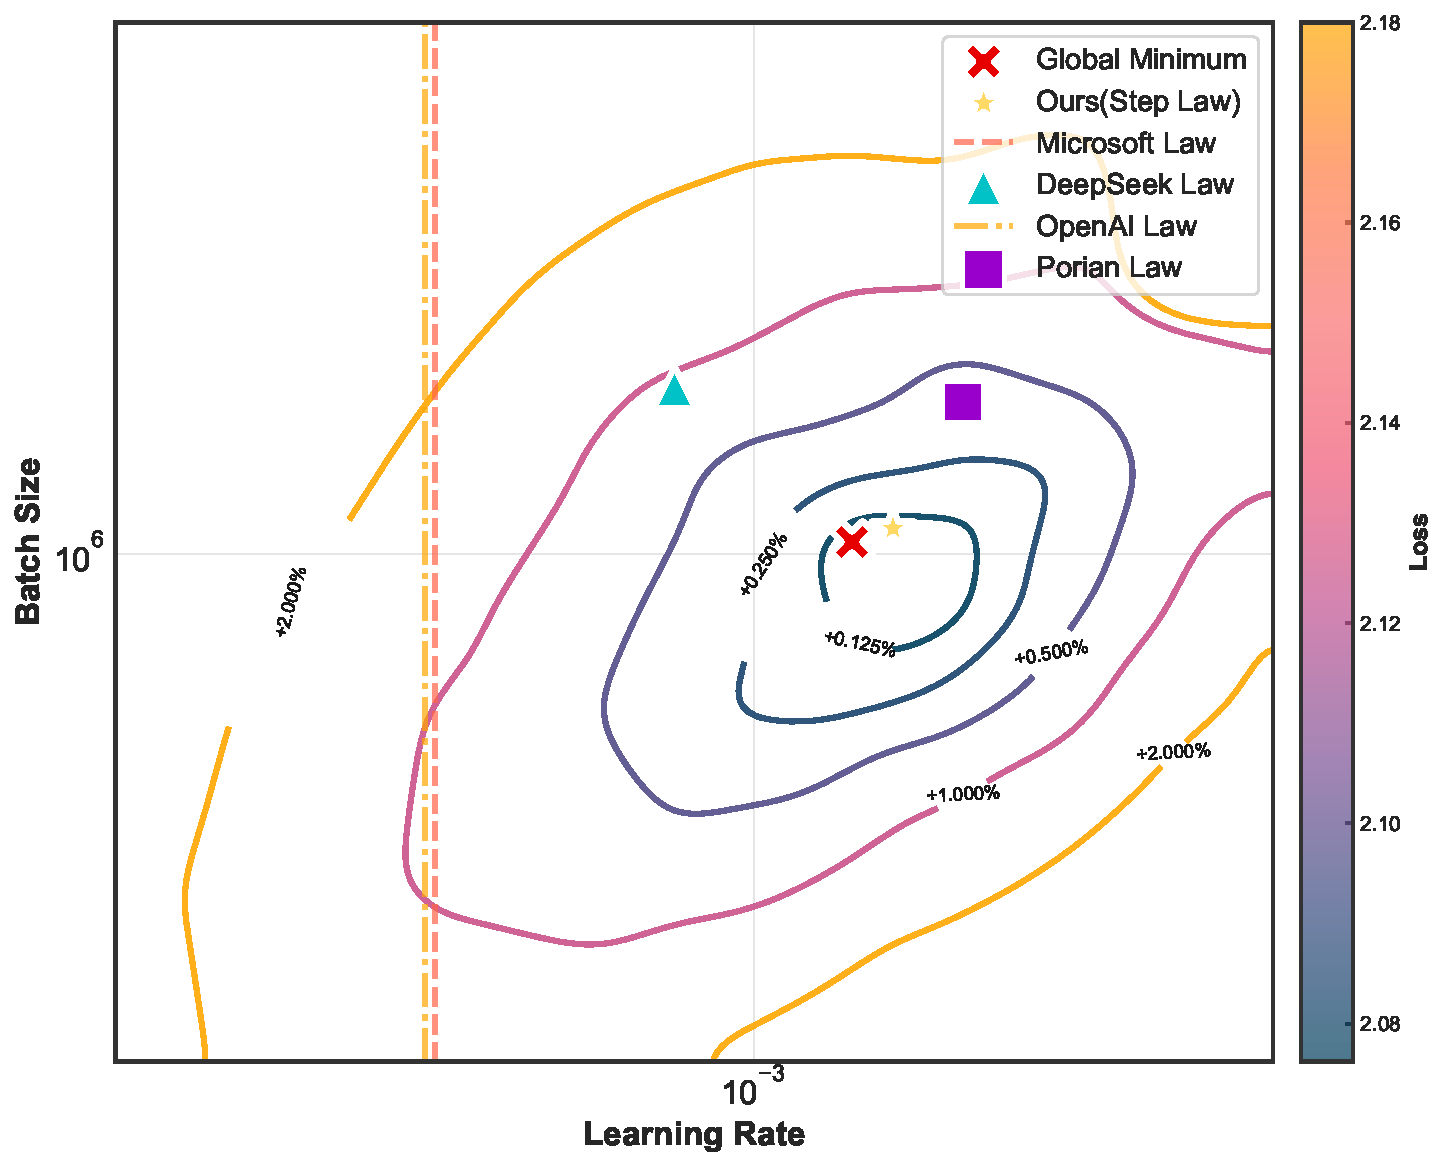
\includegraphics[width=0.5\textwidth]{pics/N1073741824_D100000000000_config_space.pdf}}
            \vskip -5pt
            \caption{This plot shows the hyperparameter space for a model with 1 billion (B) parameters trained on 100B tokens. We trained 120 LLMs from scratch with different learning rate (LR) and batch size (BS) combinations, obtaining contour lines and global optimal points based on real data. Optimal points represent the lowest training loss for each LR and BS pair, while contour lines depict the relative loss differences from these optima. Our Step Law predicts the optimum with the highest accuracy compared to other methods, nearly matching the global optimal points.}
            \label{fig:firt_pic_baselines_compare}
            \vskip -30pt
        \end{center}
    \end{figure}
    
    
    The success of LLM pretraining heavily depends on hyperparameter settings, particularly
    the learning rate and batch size. Suboptimal configurations can lead to
    various issues: excessive learning rates may cause training divergence,
    while insufficient rates slow down progress \cite{Shen2024,Wen2024}; similarly, batch size must
    balance computational efficiency and model quality \cite{Perko2023,Filatov2024,McCandlish2018}. Traditional grid
    search becomes prohibitively expensive at scale, leading researchers to rely
    on hyperparameter transfer methods extrapolating optimal configurations
    from smaller-scale experiments to larger ones \cite{Yang2020,Yang2023}.
    
    \begin{equation}
    \begin{aligned}
        \eta(N, D) & = 1.79N^{-0.713}D^{0.307}  \\
        B(D)       & = 0.58D^{0.571}           %\eta(N, D) &= 1.79 N^{-0.713}D^{0.307} \\
        \label{stepai}
    \end{aligned}
    \end{equation}




    Prior work in hyperparameter transfer broadly falls into two categories: theory-driven
    and data-driven approaches. In theory-driven methods, $\mu$P \cite{Yang2022}
    pioneered learning rate transfer rules across model widths, with subsequent work
    \cite{Everett2024,Lingle2024,Blake2024,Yang2023,Bordelon2023} extending these
    findings to various model depths while also revealing their limitations. In
    data-driven approaches, \citet{kaplan_scaling_2020} established foundational
    learning rate scaling laws based on model size $N$, inspiring further investigations
    \cite{Bjorck2024,DeepSeek-AI2024,Porian2024,Hu2024} into learning rate (LR) and batch size (BS) scaling for dense models. Recently, \citet{Wang2024,Ludziejewski2025} had begun exploring these
    relationships in Mixture-of-Experts (MoE) models\cite{Du2021,Fedus2021}.

    However, a significant gap remains in understanding hyperparameter transfer across
    different dimensions: data recipe, model shape, model sparsity, and data sizes
    $D$. While existing research has made progress in understanding scaling
    behavior across model sizes\cite{kaplan_scaling_2020,Halfon2024} the interaction of these other critical factors
    remains under-explored. Our work addresses this gap by empirically
    discovering universal hyperparameter (HP) scaling laws that hold across
    these varied dimensions, providing a more comprehensive understanding of optimal
    hyperparameter selection in LLM pretraining.

    \begin{figure*}[!t]
        \setlength{\abovecaptionskip}{0pt}
        \setlength{\belowcaptionskip}{10pt}
        %\vskip -0.4in
        \begin{center}
            \centerline{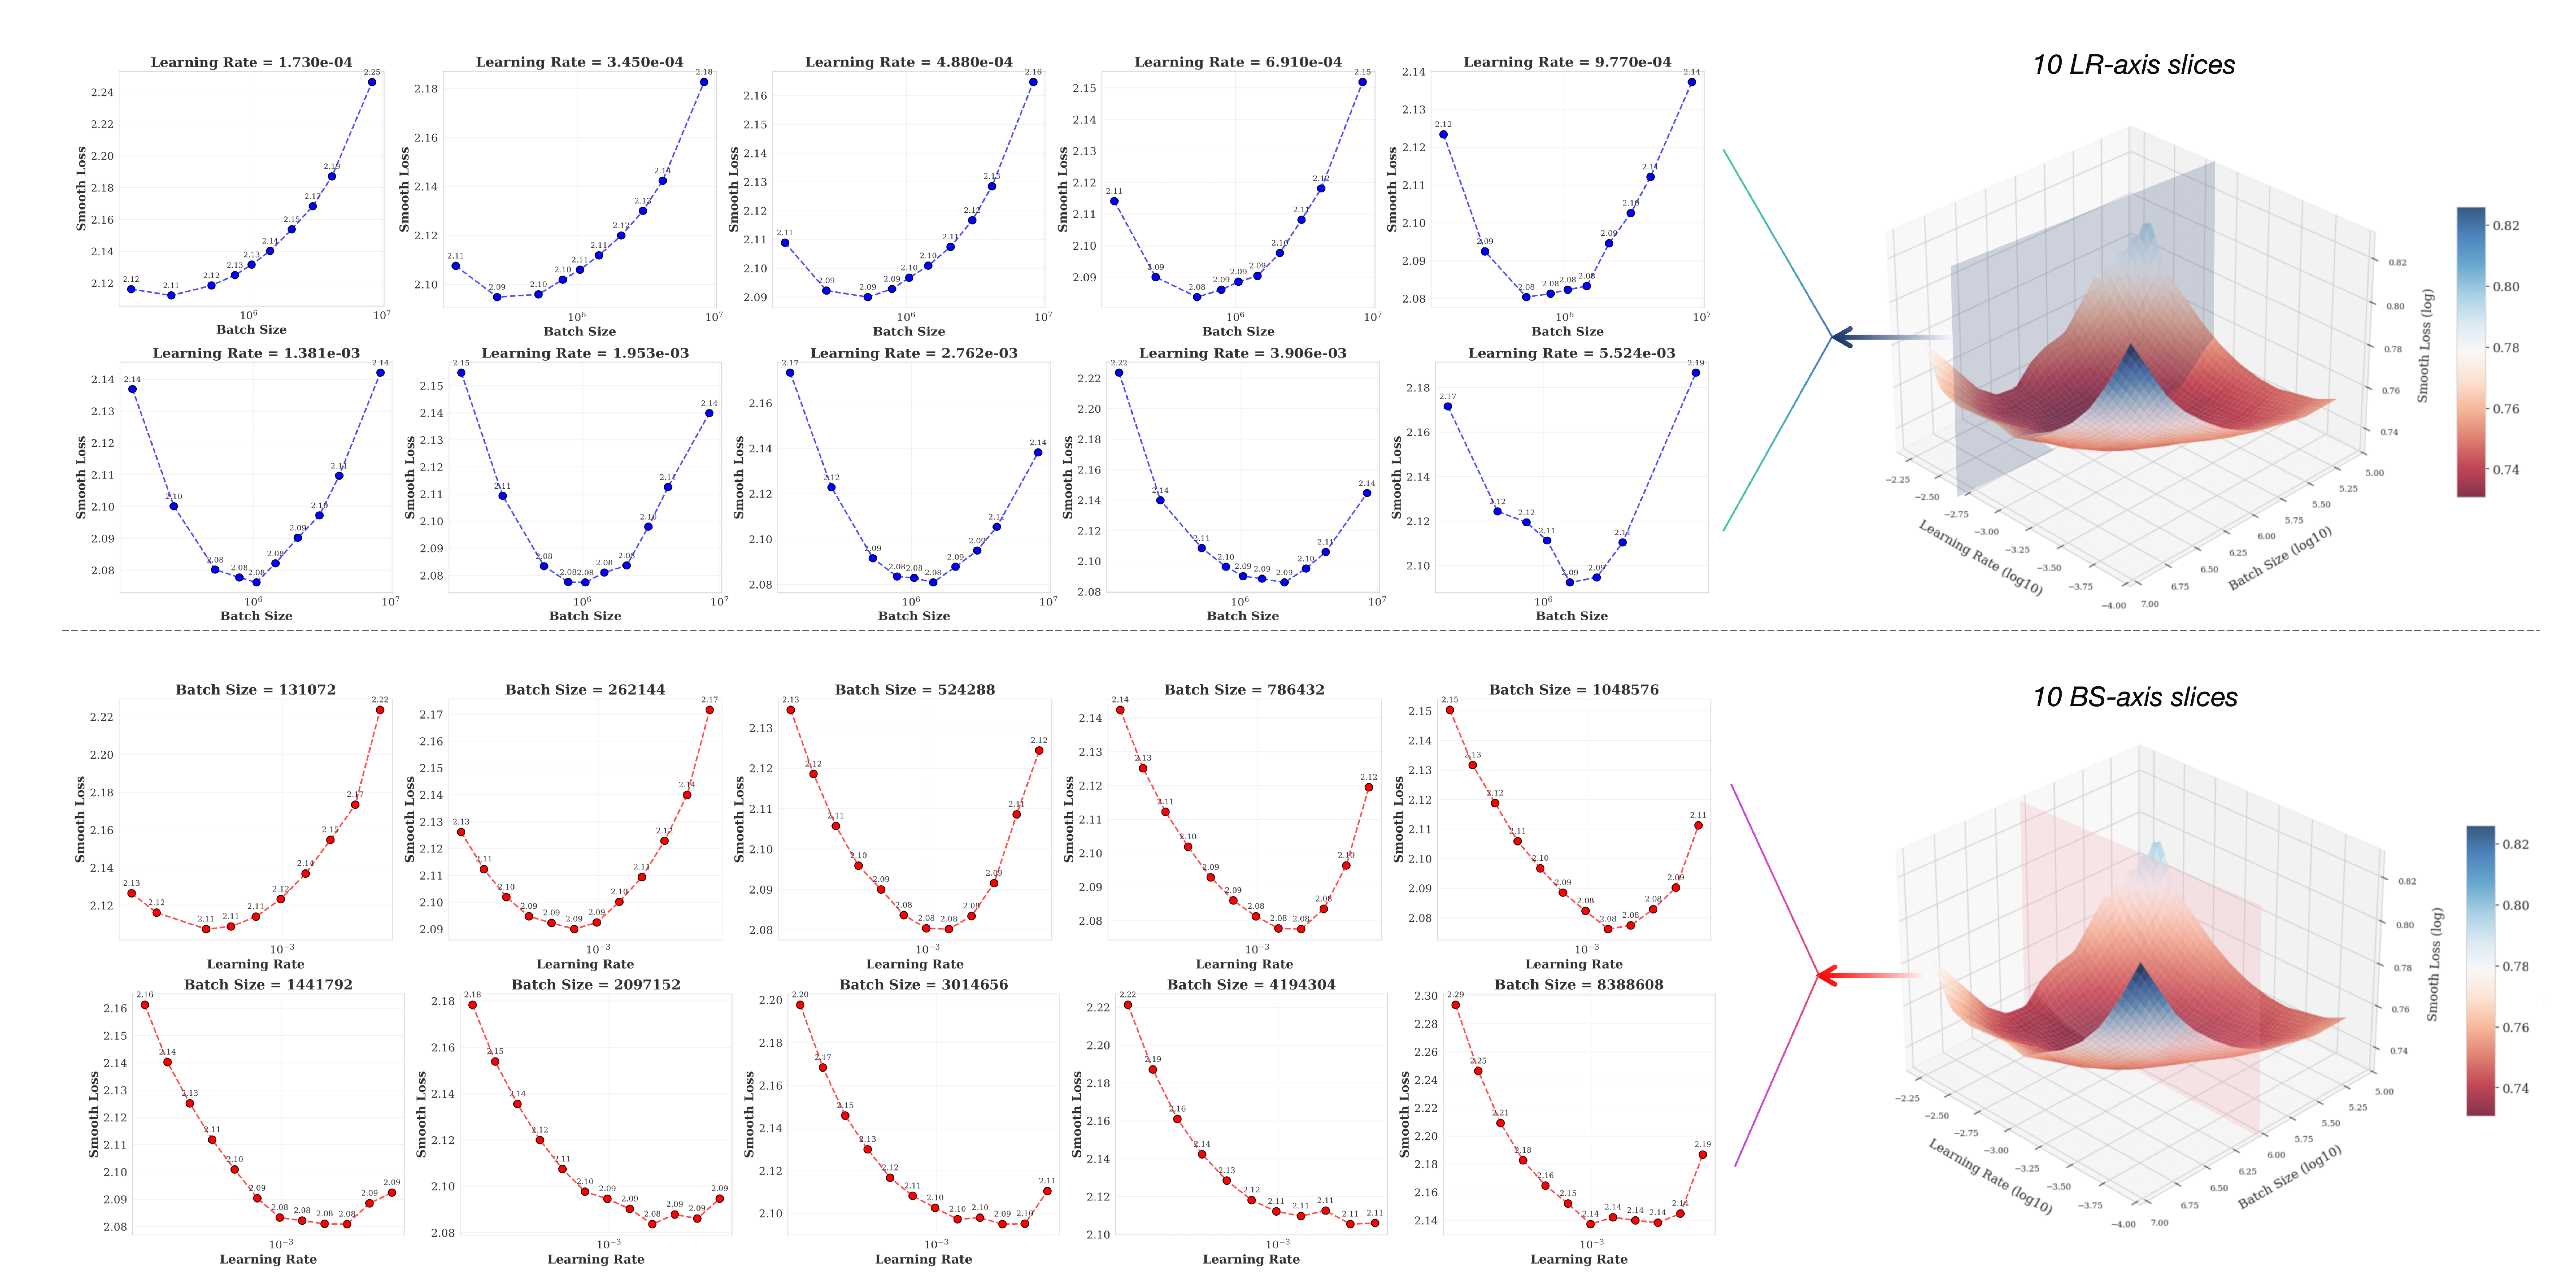
\includegraphics[width=1.0\textwidth,clip]{pics/convex.pdf}}
            \caption{Learning Rate vs. Batch Size Loss Landscape Analysis for 1B Model (Trained on 100B Tokens): Scatter Plots and 3D Surface Visualizations of Hyperparameter Sensitivity.}
            \label{fig:Convex}
        \end{center}
        % \vskip -20pt
    \end{figure*}

    Our main contributions are as follows:

    (\rmnum{1}) We are the first to discover and demonstrate the convexity property of the loss landscape under fixed parameter count and data size conditions. This provides fundamental insights into hyperparameter optimization, as shown in Fig.~\ref{fig:Convex}.

    (\rmnum{2}) We establish the first universal and robust hyperparameter
    scaling laws for LLM pretraining, which is called Step Law. Our Empirically discovered the power-law
    relationship between optimal learning rate $\eta(N, D)$ and optimal batch
    size $B(D)$. Step Law demonstrates that the optimal batch size exhibits a primary dependence on dataset size $D$, while the optimal learning rate manifests a joint dependence on both model parameters $N$ and dataset size $D$. 
    Step Law is defined as Eq.\eqref{stepai}.
    
   
    The Step Law achieves substantially superior convergence results compared
    to baseline methods when generalized to 1 billion parameter models, as
    illustrated in Fig.~\ref{fig:firt_pic_baselines_compare}.
    Step Law provides a plug-and-play formula that eliminates extensive hyperparameter tuning efforts for industry applications.
    
    
    (\rmnum{3}) 
    We are the first to study the transferability and invariance of optimal hyperparameter scaling laws across different pretraining data distributions. We systematically analyze how optimal hyperparameter scaling laws transfer across different pretraining data distributions and model architectures. Our work pioneers the investigation into whether dense LLMs and sparse (MoE) LLMs with varying sparsity levels share common optimal hyperparameter patterns, revealing significant invariance properties between them. Through extensive grid search experiments, we validate that Step Law maintains high generalizability and robustness across different pretraining corpora distributions, model architectures, and both dense and sparse (MoE) LLMs with varying sparsity ratios.
    
    (\rmnum{4}) We conduct an unprecedented large-scale empirical study, involving:
    \begin{itemize}
        \item Extensive experimentation across 3700 model configurations, training LLMs from scratch with Dense and MoE (varying sparsity ratios), model architectures, data distributions, and hyperparameter settings.
        \item Total compute consumption approaching 1 million H800 GPU Hours (equivalent to over \$1 million), processing approximately 100 trillion tokens during training.
    \end{itemize}
    This represents the largest dataset of hyperparameter optimization results
    in the field, derived purely from empirical observations without prior assumptions.
    Training checkpoints and hyperparameter configurations will be made publicly available.

    \subsection{Notation}
    \label{sec:notation}
    We use the following notation:
    \begin{itemize}
    \item $\mathcal{L}$: Cross-entropy loss.
    \item $D$: Dataset size in tokens.
    \item $N$: Number of non-embedding parameters in the model.
    \item $\hat{N}$\footnote{$\hat{N}$ excludes embedding layer but includes the model’s head layer}: Total number of parameters in the model .
    \item $C$: Compute budget in FLOPs.
    \item $N_{{layer}}$: Number of layers in the Transformer model.
    \item $d_{ff}$: Dimension of the feed-forward network hidden layer in the Transformer.
    \item $d_{{model}}$: Hidden dimension of the Transformer model.
    \item $N_{{head}}$: Number of attention heads in the Transformer model.
    \item $\eta(N, D)$: Optimal peak learning rate for a given parameter count $N$ and dataset size $D$.
    \item $B(N, D)$: Optimal batch size (in tokens)  for a given parameter count $N$ and dataset size $D$.
    \end{itemize}

    
    \section{Related Works}

    Hyperparameter transfer, which involves extrapolating optimal settings from smaller
    to larger models, has become essential for efficient large-scale training. Among
    these, learning rate (LR) and batch size (BS) are particularly crucial
    hyperparameters that substantially influence LLM pretraining performance\cite{Halfon2024}. Research on optimal learning rate and batch size selection broadly falls into two categories: theory-driven and data-driven approaches.

    % theory driven
    In theory-driven approaches, $\mu \text{P}$ \cite{Yang2022}
    established foundational learning rate transfer rules for varying model
    widths, though this required specific modifications to initialization and attention
    mechanisms. However, the $\mu \text{P}$ framework and its extensions \cite{Yang2022,Everett2024,Lingle2024,Blake2024,Yang2023,Bordelon2023}
    are limited in scope, lacking guidance for learning rate adaptation across different
    data distributions, model architectures, sparsity levels, and data sizes. Additionally,
    these works do not address batch size optimization.

    %Data driven
    In data-driven approaches, a fundamental principle in deep learning is that larger
    models require smaller learning rates to ensure training stability and convergence.
    \citet{kaplan_scaling_2020} formalized this relationship, expressing
    learning rate as a function of model size. \citet{Bjorck2024} incorporated data size
    dependency by proposing $LR(N,D)=CN^{-\alpha}D^{-\beta}$. Batch size
    optimization is equally important for balancing convergence and
    computational efficiency. While several approaches followed \citet{kaplan_scaling_2020}'s
    framework, they face limitations: \citet{Wang2024,Hu2024} derived batch size
    based on expected loss but require prior knowledge of model behavior; \citet{Porian2024}
    refined scaling laws across two datasets but only considered model size,
    setting final learning rates at 0.1\% of peak values. 
    
    Notably, both early work
    \cite{McCandlish2018} and recent Critical Batch Size (CBS) analysis \cite{zhang2024}
    support our empirical finding that optimal batch size primarily depends on dataset
    size rather than model size, with CBS establishing a theoretical upper bound
    for this relationship. DeepSeek-LLM \cite{DeepSeek-AI2024}, while
    comprehensive in its approach using IsoFLOP \cite{hoffmann_training_2022}, is
    constrained by its fixed compute budget assumption.

    Our research advances these findings by demonstrating that model size and dataset
    size are sufficient predictors of optimal hyperparameters. We validate these
    scaling rules across diverse architectures, including variations in model sparsity,
    data distributions and model shape.


    \begin{figure*}[!t]
        \centering
        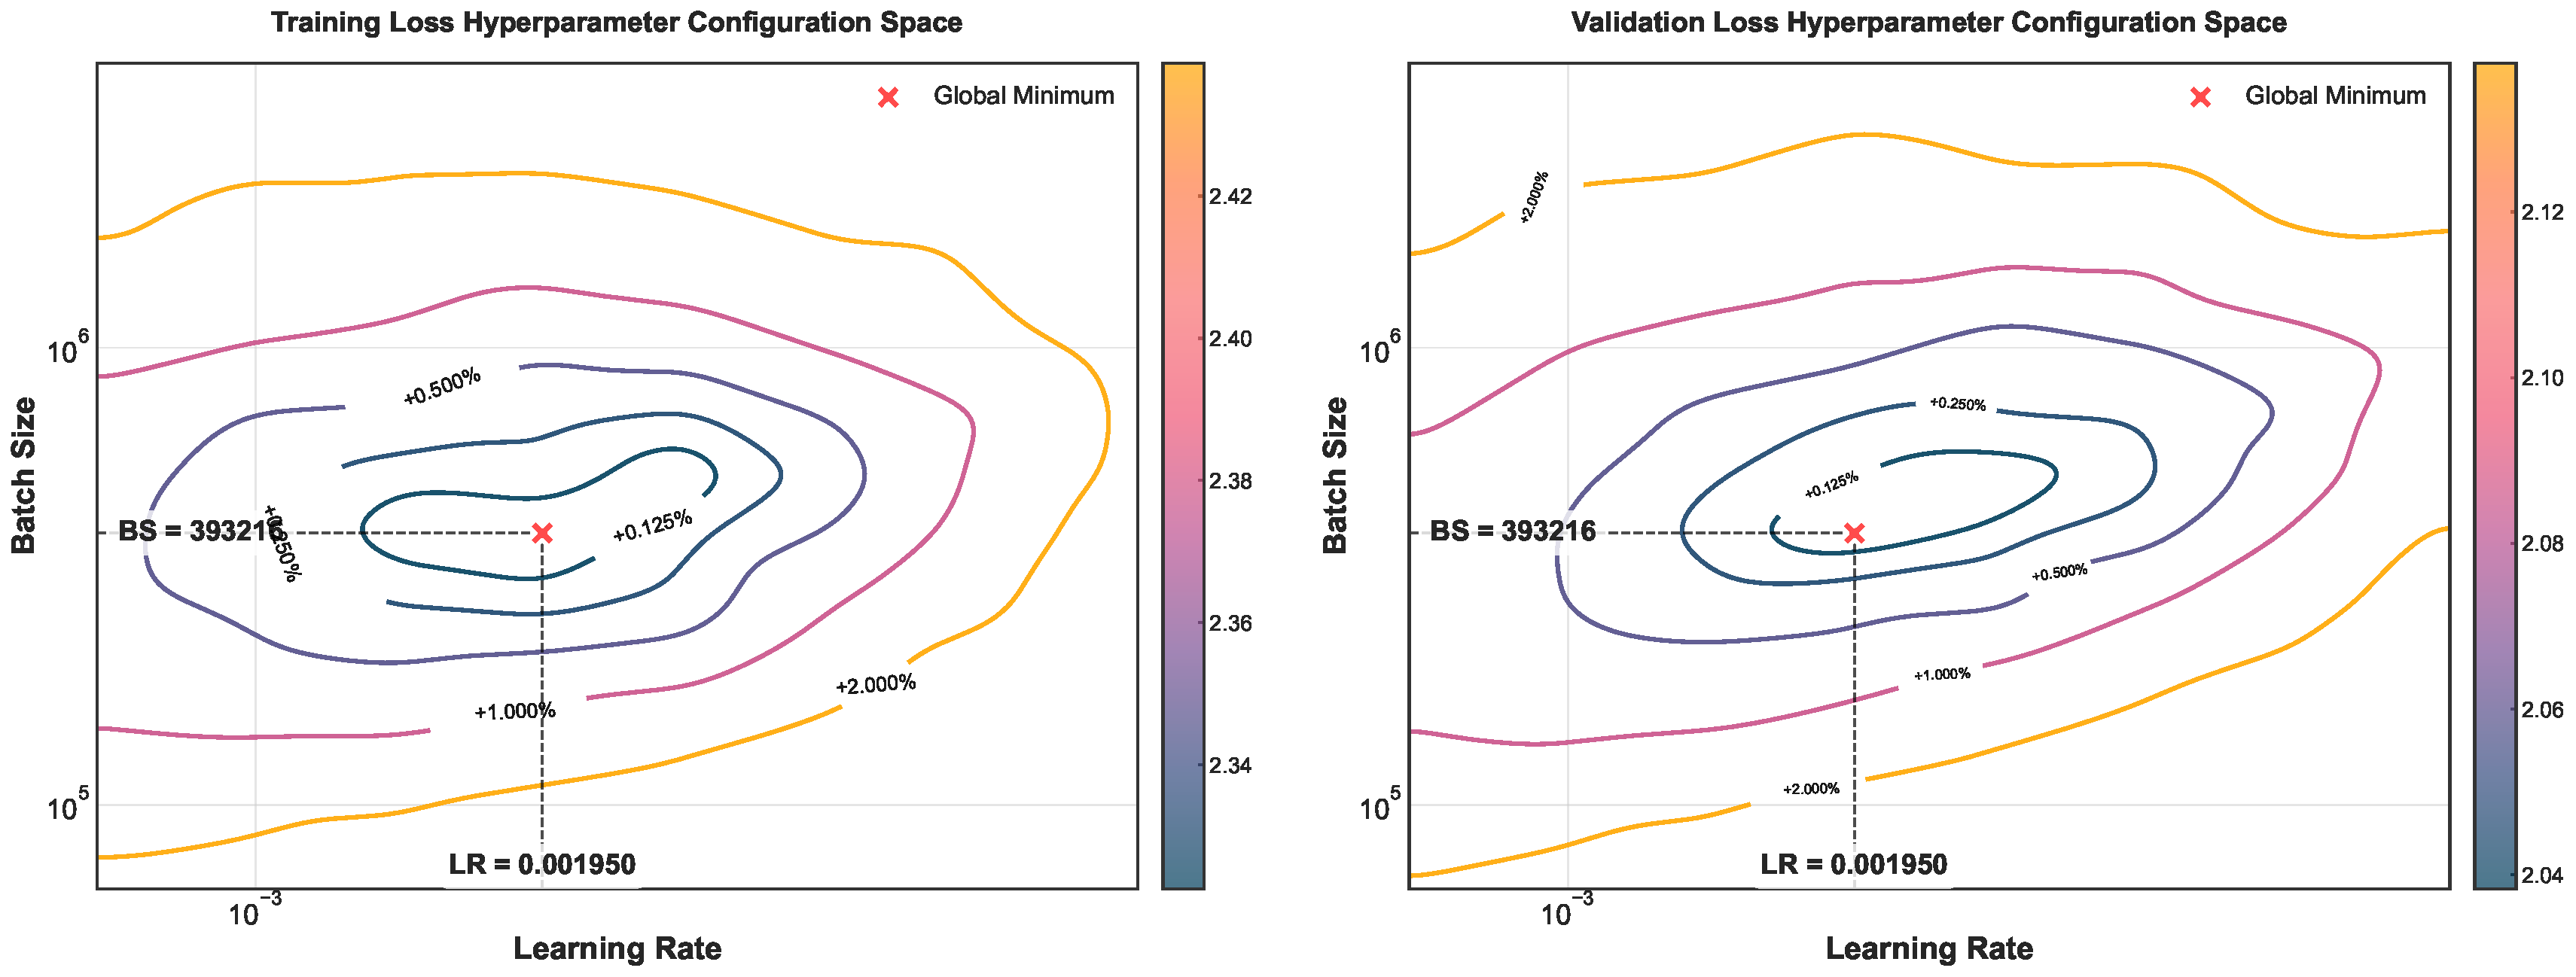
\includegraphics[width=1.0\textwidth]{pics/N429260800_D22700000000_bpc_loss_compare.pdf}
        \caption{\textbf{Contour plots of training loss (left) and validation loss} (right) across hyperparameter configurations. Both plots share the global minimum ({\color{red}\ding{55}}) at batch size 393,216 and the learning rate of 0.001950. }
        \label{fig:loss_bpc_heatmaps}
    \end{figure*}

    \section{Problem Setup}

    \subsection{Preliminaries}
    \label{preliminaries} For training LLMs, the comprehensive performance
    metric is defined as
    \begin{equation}
        \mathcal{L}(\mathbb{A}, \mathbb{D}, N, D, \text{LR}, \text{BS}),
    \end{equation}
    where $\mathbb{A}$, $\mathbb{D}$, $N$, $D$, \text{LR}, and \text{BS} represent
    the model architecture space, training data distribution, number of non-vocabulary
        parameters, number of training tokens, learning rate and batch size.

    Based on this definition, when considering specific conditions, first, given
    that both $\mathbb{A}$ and $\mathbb{D}$ are discrete variables, the performance
    metric can alternatively be expressed as
    % First, given that both $\mathbb{A}$ and $\mathbb{D}$ are discrete variables, the performance metric can alternatively be expressed as
    \begin{equation}
        \mathcal{L}_{\mathbb{A},\mathbb{D}}(N, D, \text{LR}, \text{BS}). \label{eq:fix_A_D}
    \end{equation}

    Furthermore, for given $N$ and $D$, Eq.\eqref{eq:fix_A_D} can be transformed
    into
    \begin{equation}
        \begin{aligned}
             & \mathcal{L}_{\mathbb{A}, \mathbb{D}, N, D}(\text{LR}, \text{BS})
        \end{aligned}
    \end{equation}
    In light of the above transformations, we can generate the following
    definition.

    \textbf{Definition 1: }\label{defin:1} (\emph{Hyperparameter Optimality}) For fixed
    architecture $\mathbb{A}$, data distribution $\mathbb{D}$, and training
    budget $(N, D)$, the optimal learning rate $\eta$ and batch size $B$ satisfy:
    \begin{equation}
        \eta, B = \mathop{\mathrm{arg\,min}}_{\text{LR}, \text{BS}}\mathcal{L}_{\mathbb{A},\mathbb{D},N,D}
        (\text{LR}, \text{BS}).
    \end{equation}

    \subsection{Experimental Settings}
    \label{exp_set}
    We train our models using language modeling
    loss on a dataset that includes web text, mathematical content, and code. The
    dataset is tokenized using a BPE \cite{Gage1994ANA} tokenizer with a vocabulary size of 65,536.

    Our model architecture uses RMSNorm \cite{Zhang2019} for pre-normalization and the SwiGLU \cite{Shazeer2020}
    activation function in the feed-forward network, without applying dropout \cite{JMLR:v15:srivastava14a}.
    We mainly use ALiBi \cite{Press2021} positional encoding. The models are initialized from scratch,
    with weights drawn from a truncated normal distribution (mean of 0, standard
    deviation of 0.02). For the output projection of attention layers and the
    $W_{2}$ component of the GLU, weights are further divided by $2 \cdot \text{layer
    depths}$ based on existing methods \cite{Touvron2023a,Touvron2023b,Grattafiori2024,DeepSeek-AI2024,Yang2024,DeepSeek-AI2024b,DeepSeek-AI2025,wang2019automatic,yuan2022unified}.

    We use the AdamW \cite{Loshchilov2017} optimizer with $\beta$ values of [0.9, 0.95], an epsilon of
    $10^{-8}$, a weight decay of 0.1, and a gradient clipping norm of 1.0. Our learning rate schedule includes a linear warmup phase over the initial 2,000 steps, followed by a cosine decay reaching a final learning rate of $10^{-5}$ for the remainder of the training. A detailed analysis and rationale for this strategy are provided in Section~\ref{fixed_final_lr}. The sequence length is set to 2,048 tokens. We conduct experiments using training data proportions aligned with Llama-2~ \cite{Touvron2023b} ( More details are described in Tab.~\ref{tab:data_recipes} ).

    The learning rate is selected from a logarithmic sequence of powers of 2, spanning exponents from -10.5 to -7.0 in regular 0.5-interval increments.
    The batch size is selected from a predefined geometric progression ranging from 32,768 to 4,194,304, where each subsequent batch size is obtained by multiplying the previous value by a constant factor of 2, maintaining an exponential growth trend. Both parameter configurations correspond to the 18 LLMs detailed in Tab.~\ref{tab:struct} in Appendix~\ref{app:struct}.

    \section{Experiments}


    \subsection{Ablations}

    \subsubsection{Evaluation metric}
    \label{Evaluation metric}


    As described in Chinchilla~\cite{hoffmann_training_2022}, smoothed training loss
    is considered an unbiased estimate of validation loss for simplicity. We operate
    under this same setting and supplement our investigation with experimental
    analysis.

    As shown in Fig.~\ref{fig:loss_bpc_heatmaps}, for the case where the
    smoothed training loss converges to the optimal value of $2.279$ ( as indicated
    by the solid red-framed line in Fig.~\ref{fig:loss_bpc_heatmaps} right) , the
    corresponding LR and BS are $1.95\times10^{-3}$ and $393,216$ respectively. This
    is the same as the position of the LR and BS corresponding to the validation
    loss converging to the optimal value of $2.038$ (as indicated by the solid red-framed line
    in Fig.~\ref{fig:loss_bpc_heatmaps} left). Moreover, the overall trend of how the smoothed training loss deviates from the optimal value with varying learning rates and batch sizes (as shown by the heatmap patterns in Fig.~\ref{fig:loss_bpc_heatmaps} right) closely mirrors the corresponding variations observed in validation loss measurements. This alignment demonstrates that the smoothed training loss provides consistent optimization guidance for learning rate and batch size selection, matching the parameter configurations that would be obtained through direct validation loss evaluation.


    \subsubsection{Loss Landscape Convexity with LR and BS}
    To investigate the property of the loss landscape with respect to learning
    rate and batch size, we conducted systematic experiments across a wide range
    of configurations under fixed model parameters $N$ and data size $D$. As
    shown in Fig.~\ref{fig:Convex}, one of our experiment settings described in
    Section~\ref{exp_set} demonstrates this property.
    % \input{lr_schedules}
    \begin{figure}[!t]
        \centering
        % \vskip -1in
        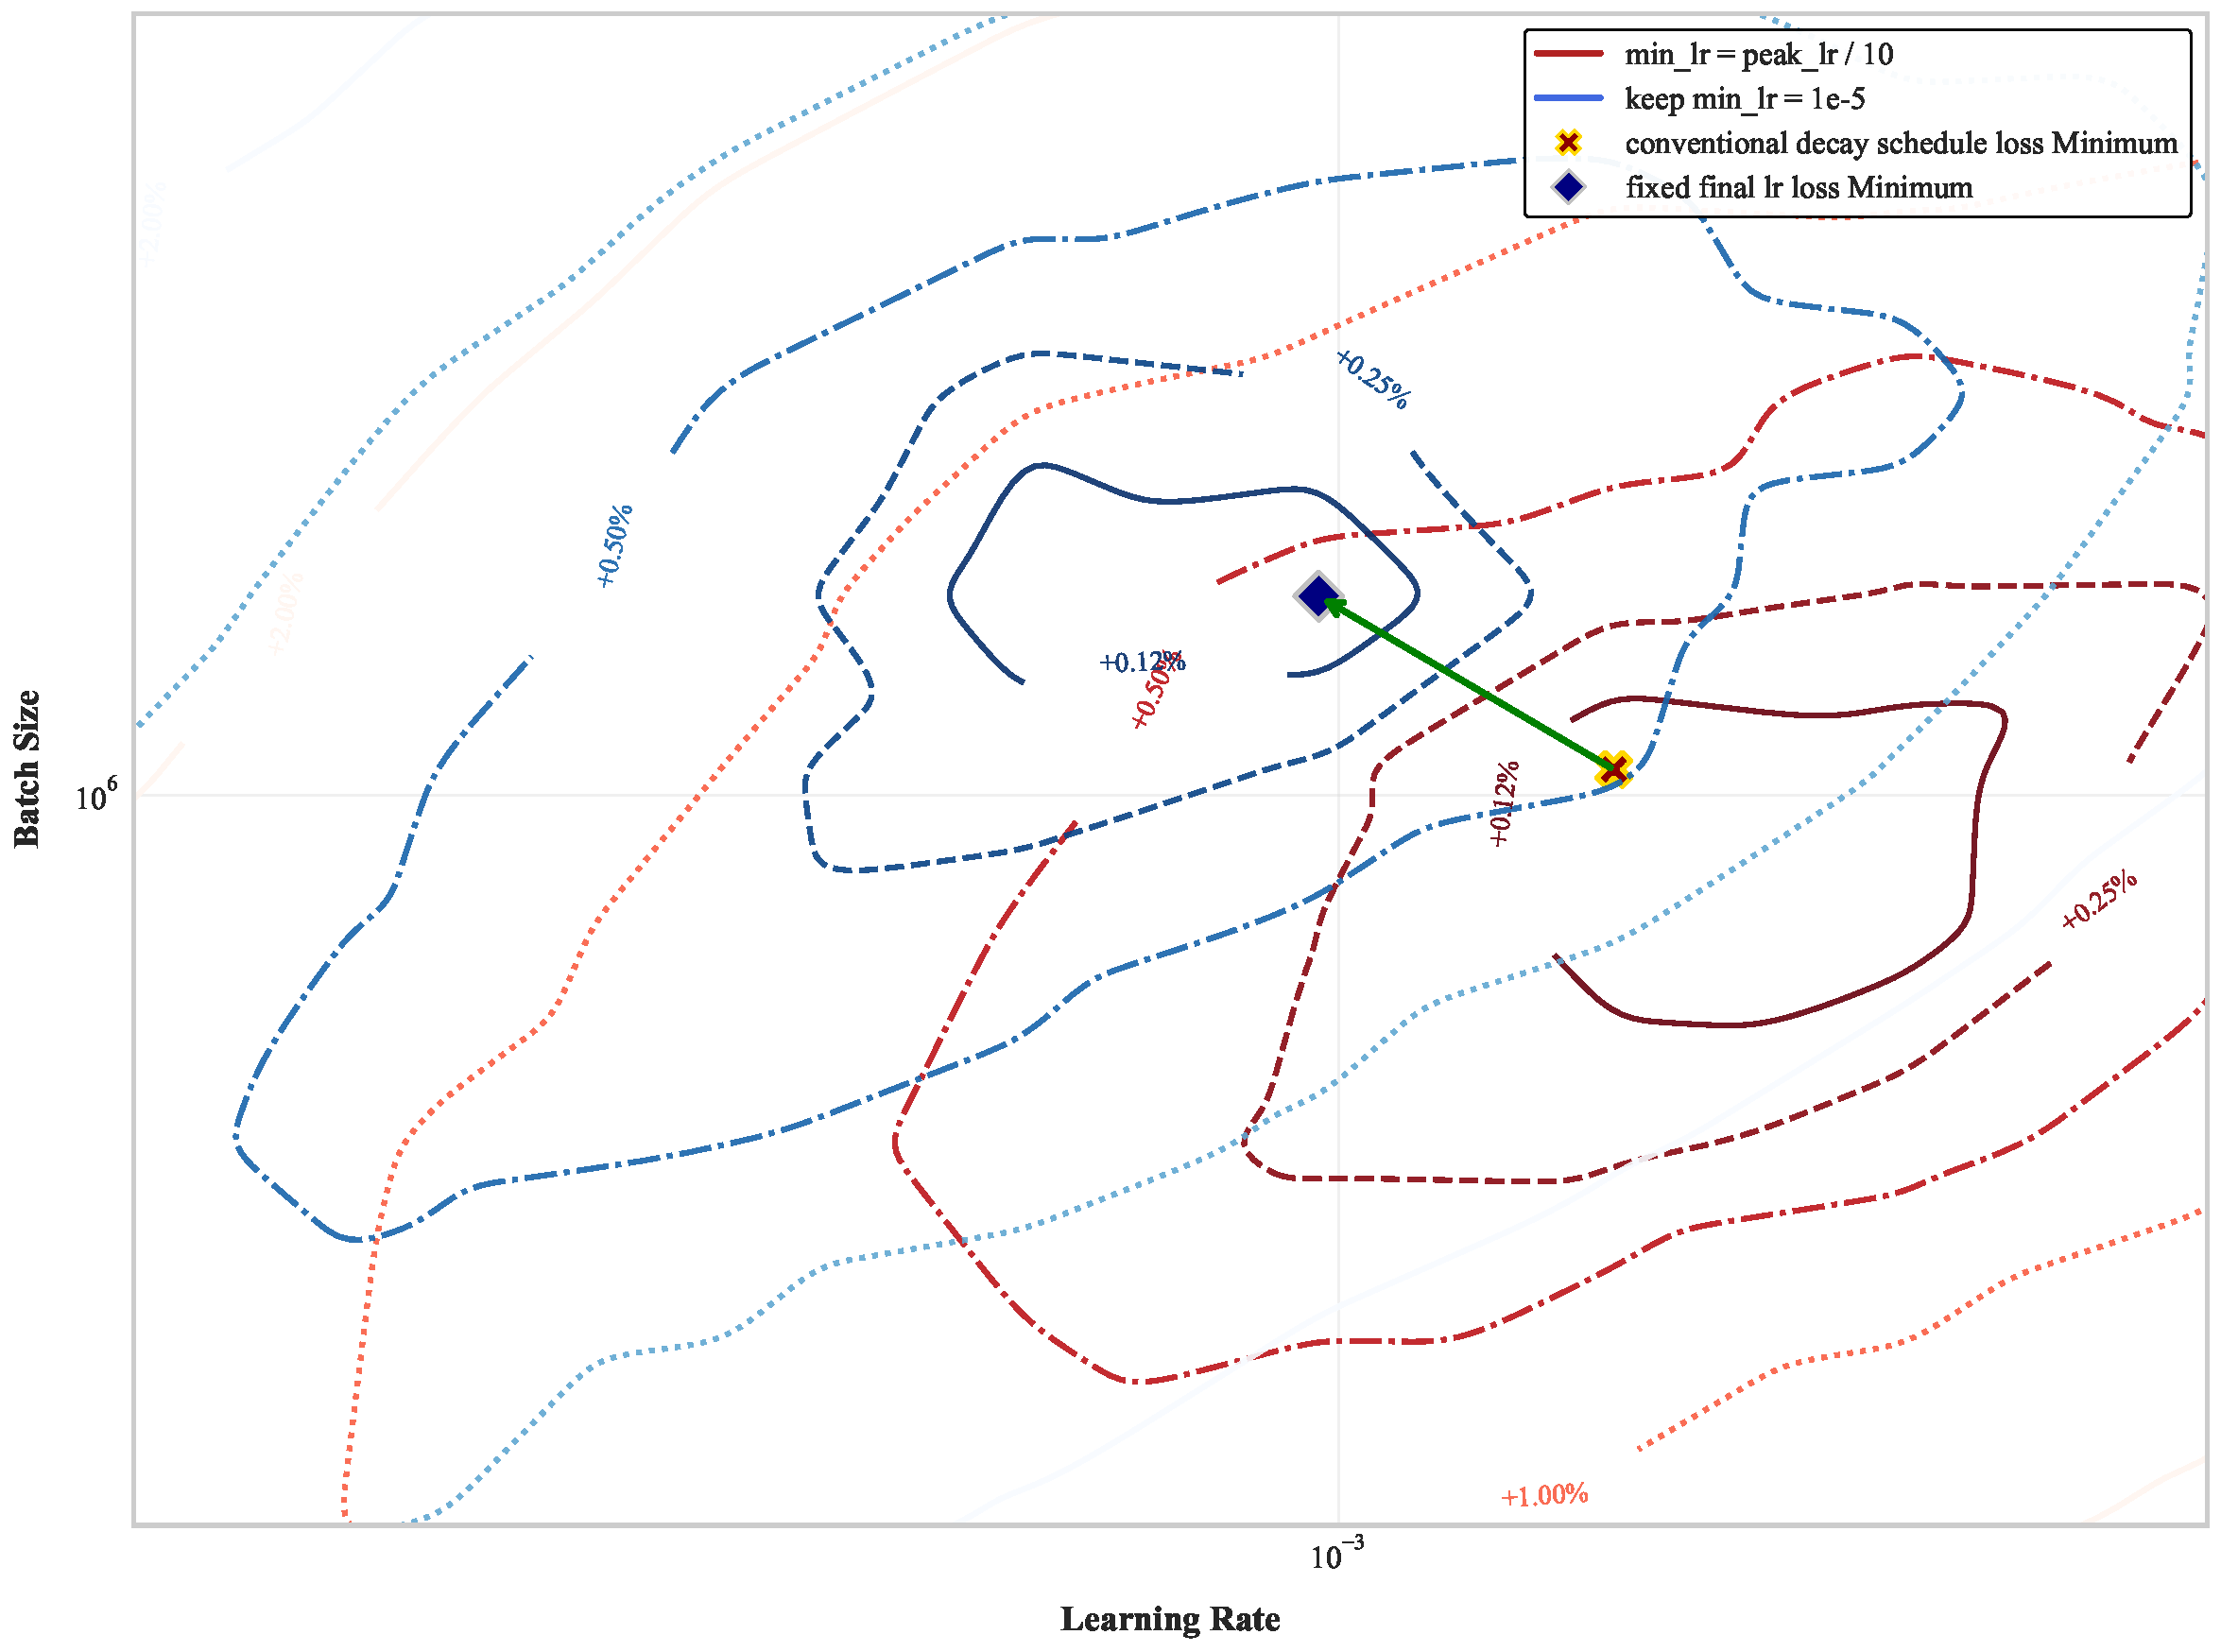
\includegraphics[width=0.45\textwidth]{pics/keep_min_lr.pdf}
        \caption{ \textbf{Comparison of learning rate schedules.} These contour
        plots illustrate two distinct learning rate schedules. \textbf{Blue
        contours} represent the \textit{conventional decay schedule}, where the
        minimum learning rate ($\min\_lr$) is set to one-tenth of the maximum
        learning rate ($\frac{\max\_lr}{10}$). \textbf{Red contours} depict our
        proposed \textit{fixed final learning rate schedule}, with a constant
        minimum learning rate of $\min\_lr = 10^{-5}$. The visualization reveals
        that the conventional decay method leads to a discernible \textbf{leftward
        bias} in the optimal learning rate range, indicated by the shift of the lowest
        loss region towards lower learning rates in the blue contours compared to
        the red.}
        \label{fig:learning_rate}
        %\caption{Comparison of learning rate schedules.}
        % \vskip -20pt
    \end{figure}

    Through extensive empirical analysis, we discovered a fundamental property
    of the loss landscape with respect to hyperparameters: both the learning rate and
    batch size exhibit convex relationships with the training loss under fixed model
    parameters and data size conditions. ( As shown in Fig.~\ref{fig:Convex} one
    of our experiment setting described in section.)

    Furthermore, we observe that the loss surface demonstrates a stable region around
    the optimal configuration, evidenced by the plateau-like behavior shown in
    Fig.~\ref{fig:loss_bpc_heatmaps}. This stability provides practical
    tolerance for small deviations in hyperparameter selection while maintaining
    near-optimal performance.

    These properties form the theoretical foundation for our subsequent
    development of scaling laws and validate their applicability across
    different architectural configurations.
    \subsubsection{Fixed Final Learning Rate Strategy}
    \label{fixed_final_lr}

    We investigated two approaches for the final minimum learning rate ($\min\_lr$):
    the conventional decay schedule ($\min\_lr = \frac{\max\_lr}{10}$)\cite{Brown2020,Jin2023,Touvron2023a,Touvron2023b,biderman2023pythiasuiteanalyzinglarge,workshop2023bloom176bparameteropenaccessmultilingual,Shen2024}, and our proposed
    fixed schedule ($\min\_lr = 10^{-5}$). Using 1B model training for 80B
    tokens, we compared these schedules across various LR and BS.

    Fig.~\ref{fig:learning_rate} presents comparative heatmaps of the final training
    loss. We observe that compared to using a fixed final learning rate, setting it as max\_lr/10 shows distinct optimal hyperparameter points and an overall left-skewed distribution of suboptimal learning rate and batch size combinations. We analyze that this is because, for the relatively high peak learning rates, conventional schedules result in disproportionately large minimum learning rates, which adversely affects the final stages of training and prevents the loss from converging to better local optima.

    As can also be seen in Fig.~\ref{fig:firt_pic_baselines_compare}, aside from Porian Law, which converges the min\_lr to a sufficiently small value, the optimal learning rates calculated by other traditional learning rate decay schedules all exhibit varying degrees of a left-skew issue.
    

     This aligns with advanced training practices which suggest that the minimum learning rate significantly impacts the loss. This phenomenon is unfavorable for fitting our scaling laws, and in practice, it is generally preferred to keep the min\_lr fixed at a relatively low value. So we adopt the fixed final learning rate strategy in our subsequent experiments.

    \begin{tcolorbox}
        [callout={Key Takeaways}]
        \begin{enumerate}[\textbullet]
            \item \textbf{Convex Loss Landscape:} The loss landscape
                exhibits convexity with respect to both learning rate and batch size. This
                convexity, coupled with a stable plateau around the optimum,
                underpins the robustness of hyperparameter selection.

            \item \textbf{Fixed Final Learning Rate Benefit:} Compared to setting a small, fixed final learning rate, the traditional decay to  max\_lr/10 causes the discovered optimal learning rate to be biased towards lower values (left-skewed).
        \end{enumerate}
    \end{tcolorbox}

    \subsection{Fitting HP Scaling Laws}
    \label{fitting_hp_scaling_law}

    \subsubsection{LR and BS with Respect to $N$ and $D$}
    \label{LR_BS_wrt_N_D}

    In accordance with Definition \ref{defin:1}, we experimentally derive the LR and BS by keeping
    other variables fixed. This section focuses on elucidating the relationships between these empirically determined hyperparameters and $N$ and $D$. For the parameter count $N$, we set up seven experiments spanning 60M, 120M, 210M, 270M, 430M, 540M, and 1B parameters. As demonstrated in Fig.~\ref{fig:diff_N_LR_BS}, our experiments reveal a positive correlation between optimal LR and BS and the data scale $D$ for each value of $N$. Furthermore, we conducted experiments across five different data scales $D$: 2B, 4B, 8B, 20B, and 100B tokens. Notably, we specifically reserved the 1B parameter and 100B token settings as test points to validate our findings, as discussed in Section~\ref{sec:validation}.
    As visualized in Fig.~\ref{fig:diff_D_LR_BS}, we find that for each data scale
    $D$, the optimal LR increases with model size $N$. Notably, our findings
    indicate that optimal BS is largely independent of $N$. Based on these experimental
    observations, we will present and fit the Hyperparameter (HP) scaling law
    formulations in Section~\ref{scaling_law}.

    %\includegraphics[width=0.5\textwidth]
    \begin{figure}[!t]
        \centering
        \centerline{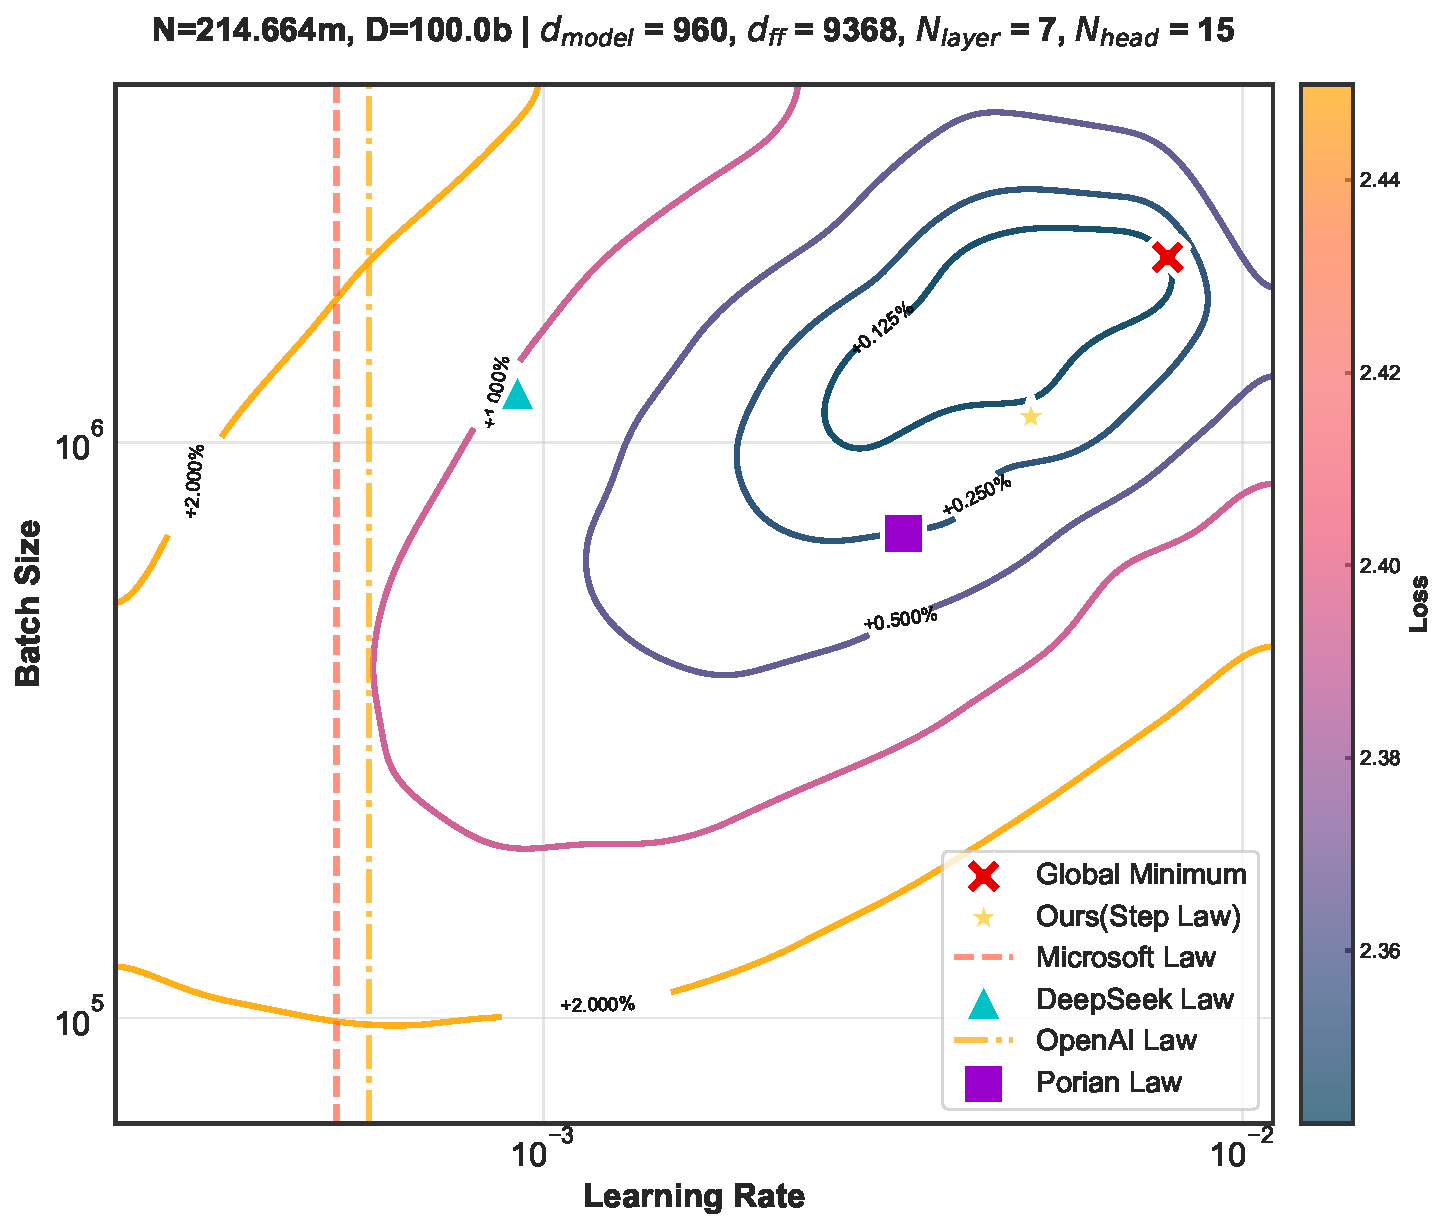
\includegraphics[width=0.5 \textwidth,trim=0 0 0 40,clip]{compare_pics/0.pdf}}
        \caption{The Illustration of Hyperparameter Configuration Space for 210M
        model parameters and 100B tokens.}
        \label{fig:compare_0}
    \end{figure}


    \subsubsection{Scaling Laws}
    \label{scaling_law}

    Building upon the insights gained from Section~\ref{LR_BS_wrt_N_D}, we delve
    into the scaling behavior of optimal hyperparameters. Specifically, we investigate
    how the optimal LR scales with $N$ and $D$, and how the optimal BS scales with $D$.
    Our empirical observations, particularly when visualized on a log-log scale, reveal a strong linear trend, suggesting a power-law relationship. Based on this, the scaling law for hyperparameters can be
    described by the following power-law relationships:
    \begin{equation}
    \begin{aligned}
        \eta(N, D) & = c N^{\alpha}D^{\beta},  \\
        B(D)       & = d D^{\gamma}
        \label{eq:scaling_law_lr_bs}
    \end{aligned}
    \end{equation}

    where the parameters $c, \alpha, \beta, d$, and $\gamma$ are five constants,
    the values of which will be determined through fitting in Section~\ref{fitting_methods}.
    It is particularly noteworthy that our proposed scaling law demonstrates significant
    generality, meaning it is applicable across diverse architectures
    $\mathbb{A}$ and data distributions $\mathbb{D}$. This aspect of generality will
    be further elaborated upon in Section~\ref{Universal_HP_law}.


    \begin{table}[h!]
        \centering
        \footnotesize
        \caption{Fitted power-law coefficients for hyperparameter scaling laws}
        \label{tab:parameters}
        \begin{tabular}{lccccc}
            \toprule \textbf{Parameter}           & $\alpha$ & $\beta$ & $\gamma$ & $c$  & $d$  \\
            \midrule \textbf{Fitted value}        & -0.713   & 0.307   & 0.571    & 1.79 & 0.58 \\
            \bottomrule \label{hp_result}
        \end{tabular}
    \end{table}

\begin{figure*}[!t]
    \centering
    \begin{subfigure}[t]{0.98\textwidth}
        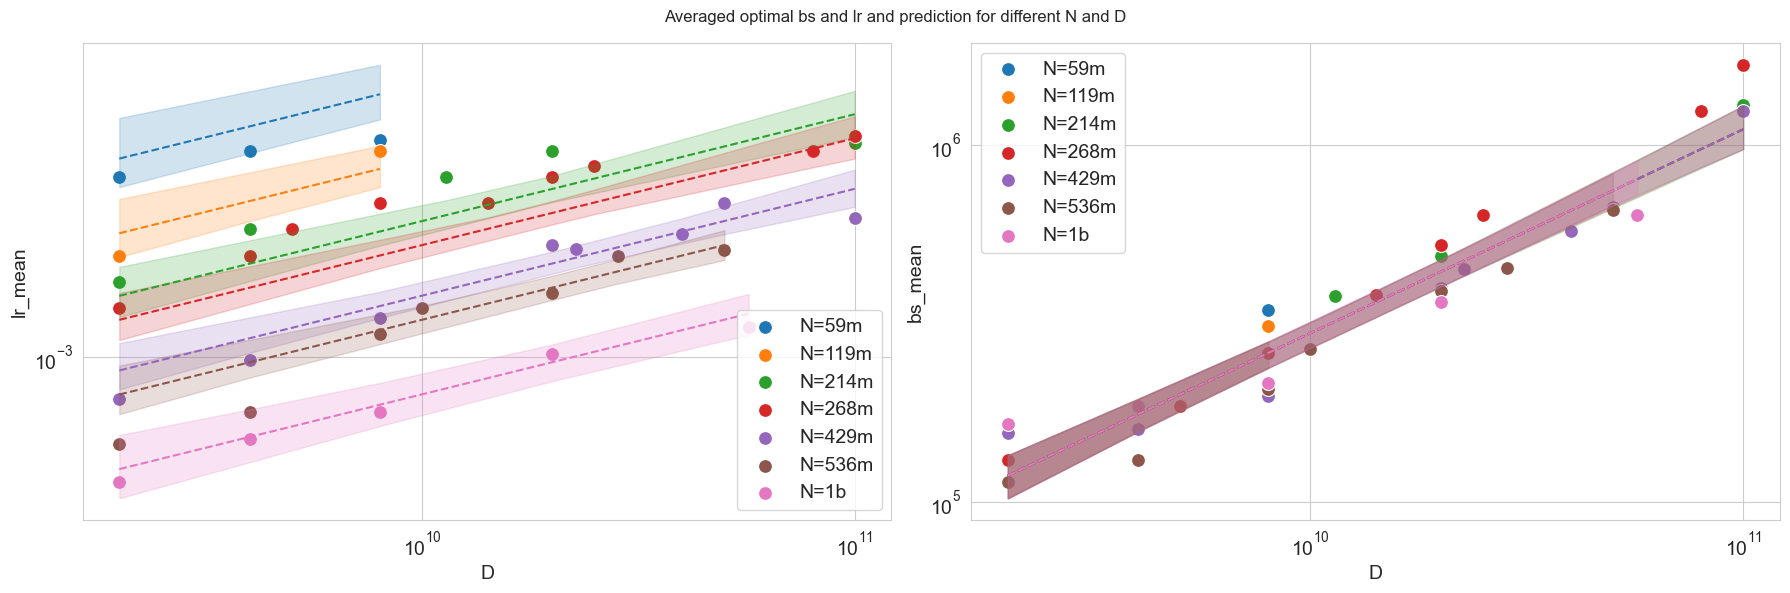
\includegraphics[width=\linewidth]{pics/1004_lr_bs_D_forN.png}
        \caption{Scaling laws with $D$ for different $N$}
        \label{fig:diff_N_LR_BS}
    \end{subfigure}
    \hfill
    \begin{subfigure}[t]{0.98\textwidth}
        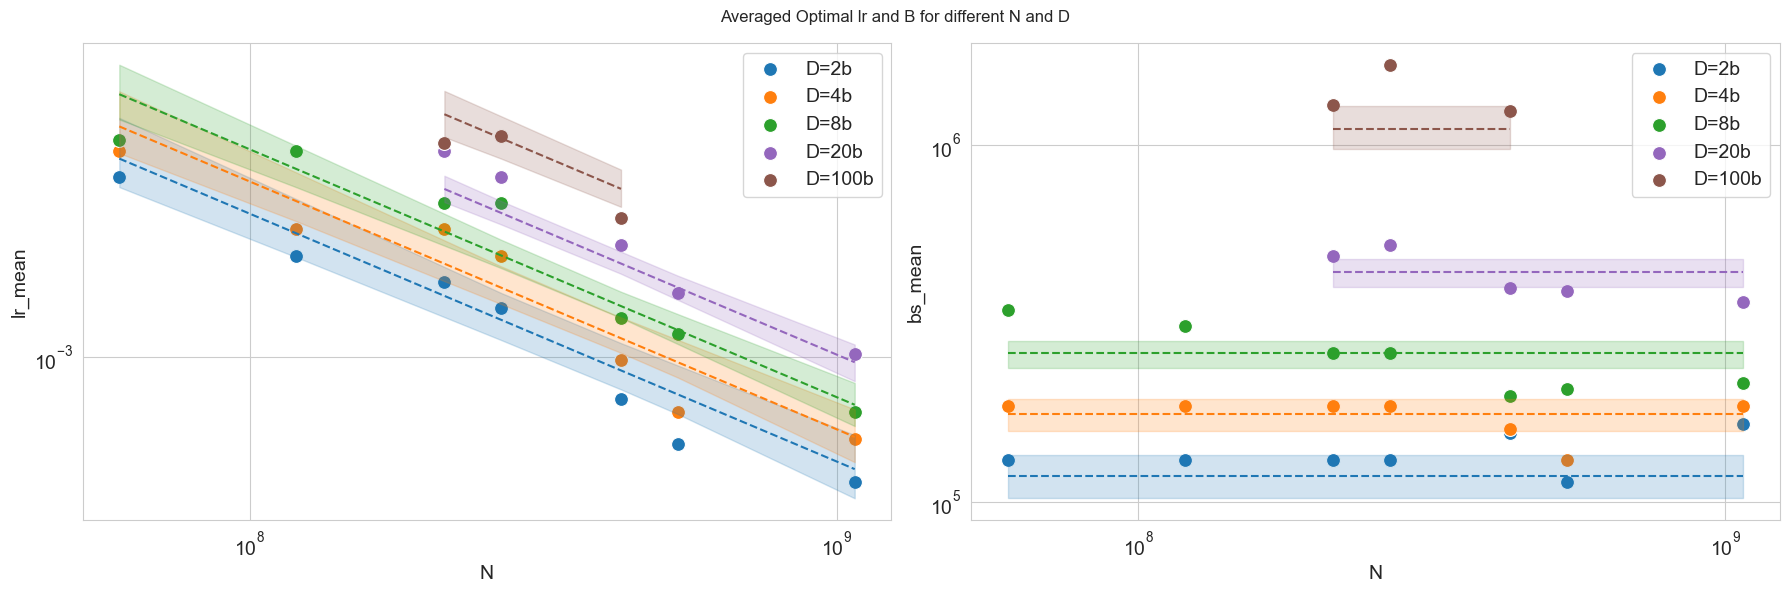
\includegraphics[width=\linewidth]{pics/1004_lr_bs_N_forD.png}
        \caption{Scaling laws with $N$ for different $D$}
        \label{fig:diff_D_LR_BS}
    \end{subfigure}
    \caption{
    (a) Scatter points indicate empirical optimal learning rate vs. batch size for model scale $N$;
    (b) Analogous results for dataset scale D.
    Curves show our hp-scaling law predictions, with shaded regions representing parameter uncertainty bounds from the sampling-based fitting strategy.
    Both plots use double logarithmic scaling (1912 training samples).
    }
    \label{fig:laws}
\end{figure*}


    \subsubsection{Fitting Methods}
    \label{fitting_methods}

    Building upon the HP scaling law from Section~\ref{LR_BS_wrt_N_D}, we
    transform the power laws in Eq.~\eqref{eq:scaling_law_lr_bs}
    into the linear form:
    \begin{align}
        \log \eta & = \log c + \alpha \log N + \beta \log D \label{eq:log_lr} \\
        \log B    & = \log d + \gamma \log D \label{eq:log_bs}
    \end{align}
    In this way, we can employ Ordinary Least Squares to fit the unknown
    parameters $\log c, \alpha, \beta, \log d$ and $\gamma$. Specifically, we
    set up 7 groups of experiments with different $N$ and $D$ as shown in Appendix~\ref{app:struct}.
    Following~\cite{hoffmann_training_2022}, we fit the optimal LR and BS with
    the experimentally predicted LR and BS. We averaged the results of these 1000 bootstrap samples to obtain the intermediate final parameters. This averaged result is what we present in Tab.~\ref{tab:parameters}. Furthermore, the variability across these 1000 bootstrap samples is depicted as the shaded regions in Fig.~\ref{fig:laws}, providing an indication of the uncertainty associated with the fitted results. These shaded regions allow us to visually assess the robustness and confidence of the optimal LR and BS values derived from our procedure.

    

    \subsubsection{Experimental Comparison with Existing Approaches}

    \label{sec:validation}
    Since we have obtained the fitted scaling laws, we directly extrapolate them
    to the test point ($N=1$B and $D=100$B) for comparison with other methods, noting that these
    are out-of-sample extrapolations beyond the fitting range. As shown in Fig.~\ref{fig:firt_pic_baselines_compare}
    and Fig.~\ref{fig:compare_0}, our method predicts solutions closest to the global
    minimum, while other approaches (indicated by dashed lines) remain distant
    from the global minimum. This discrepancy arises because previous methods only
    considered LR fitting without jointly modeling both LR and BS. The approach in \cite{DeepSeek-AI2024} enforces a fixed compute
    budget assumption, which constrains the feasible $(N, D)$ sampling range and
    consequently reduces fitting accuracy. Additionally, as discussed in Section~\ref{fixed_final_lr},
    existing methods typically relate final LR to initial LR through a fixed
    multiplier. This assumption leads to excessively large final LRs when initial
    LRs are large, ultimately impairing convergence. While \citet{Porian2024}
    achieves comparable results to ours through similar $\mathrm{min\_lr}$
    constraints, their method exhibits instability due to incomplete consideration
    of hyperparameter interactions with model dimension $D$, particularly at the subsequent MoE experiments ~\ref{sec:moe} and data recipe experiments~\ref{sec:data}, where the $D/N$ ratios are relatively small, their methods predict learning rates and batch sizes that fall completely outside reasonable ranges, leading to training instability.

    \begin{tcolorbox}
    [callout={Key Takeaways}]
    \begin{enumerate}[\textbullet]
        \item \textbf{HP Scaling Law:} We observed that the optimal LR follows a power law with respect to both $N$ and $D$, while the optimal BS follows a power law only with respect to $D$ and remains relatively invariant to $N$. Based on these observations, we derived our formula.

        \item \textbf{Experimental Comparison:} Relative to other approaches, our approach involved a substantial resource allocation to comprehensively analyze the dependence of LR and BS on $N$ and $D$. This resulted in a marked improvement in performance.
    \end{enumerate}
    \end{tcolorbox}


    \section{Universal HP Scaling laws: Empirical Validation Across Architectural
    Heterogeneity and Data Recipes}
    \label{Universal_HP_law}
    \subsection{Topological Invariance Across Varied Model Shape}


    \begin{figure*}[!t]
        \setlength{\abovecaptionskip}{0pt}
        \setlength{\belowcaptionskip}{10pt}
        %\vskip -0.2in
        \begin{center}
            \centerline{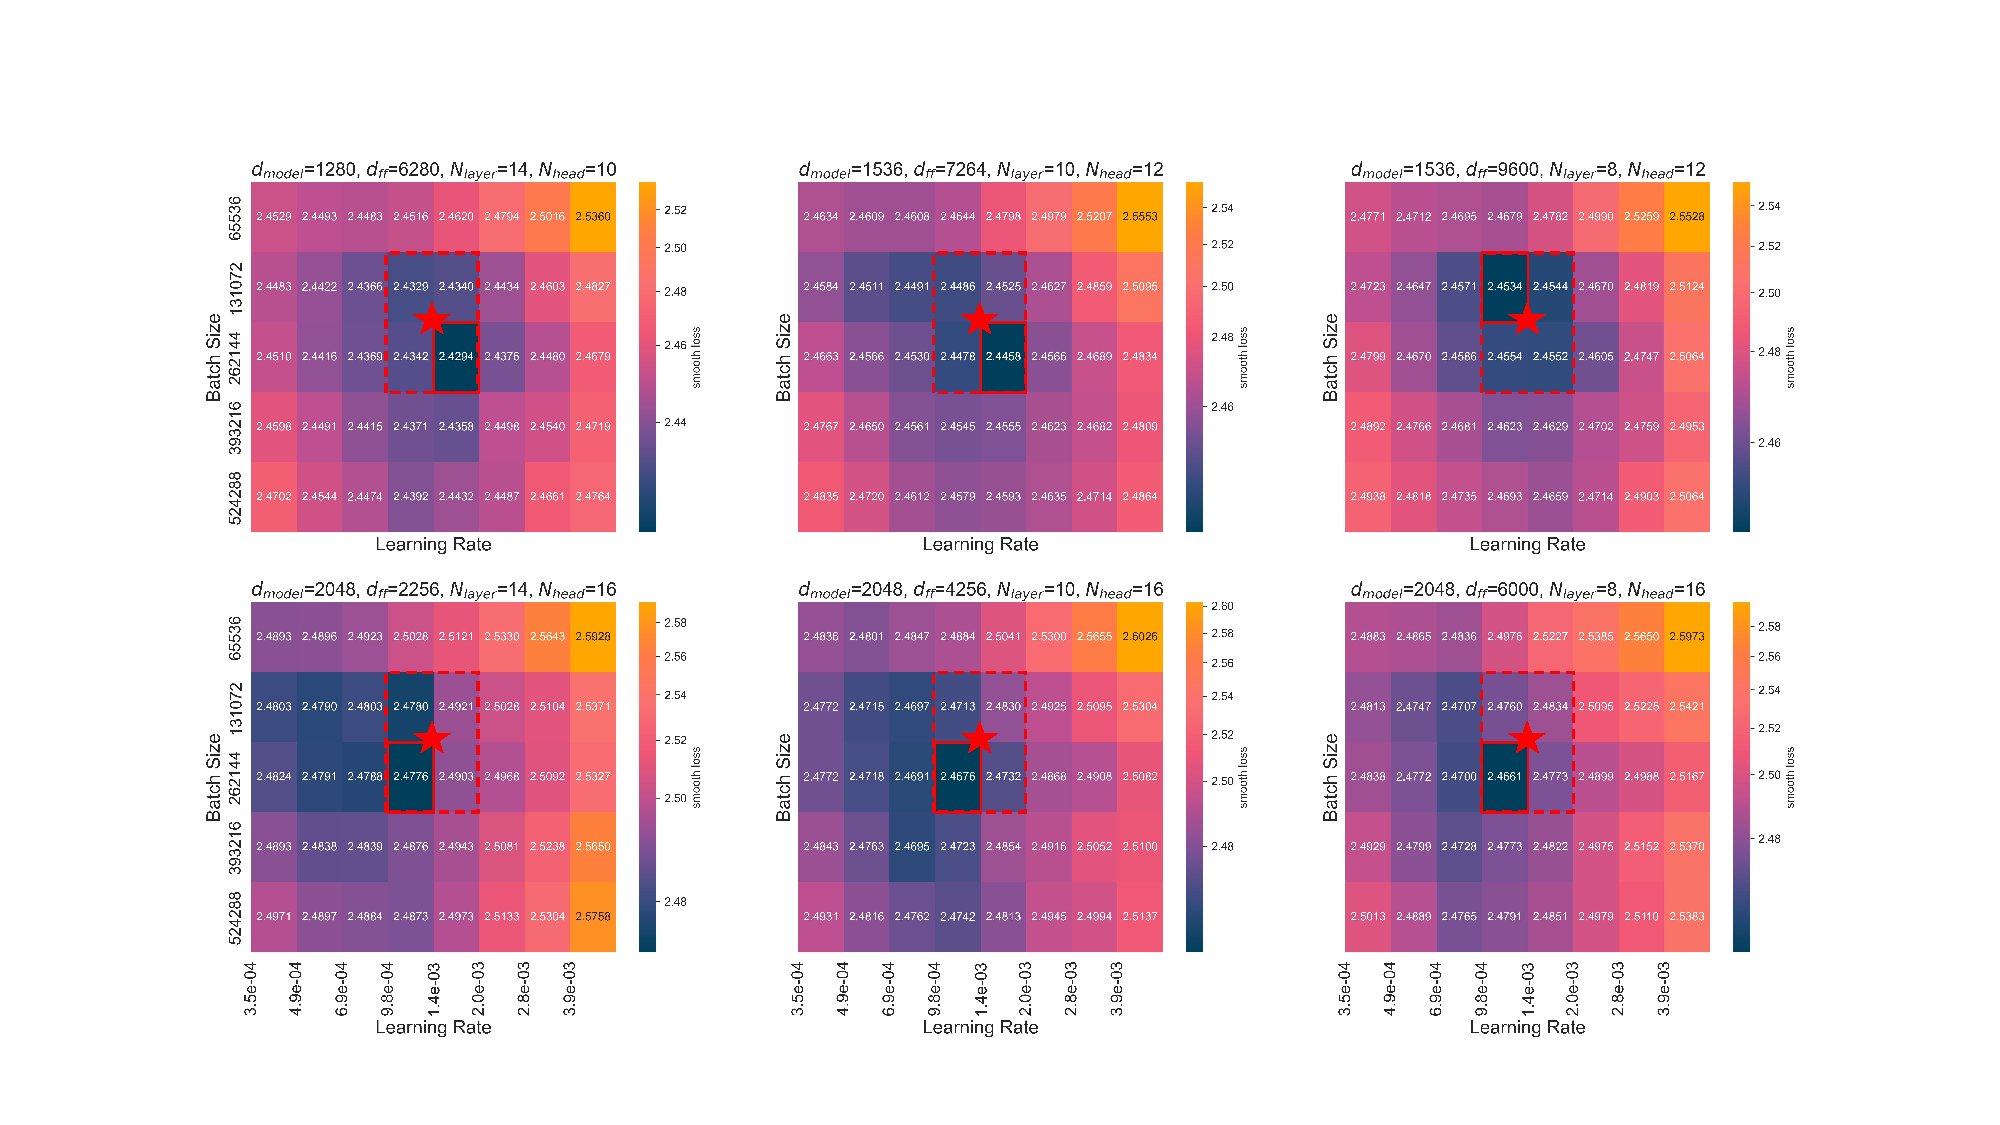
\includegraphics[width=1.0\textwidth]{pics/Topological_Invariance_in_Parameter_Scaling.pdf}}
            % \vskip -10pt
            \caption{ \textbf{Topological Invariance Across Varied Model Shape}. $d_{\text {model }}$, $d_{\mathrm{ff}}$, $N_{\text {layer}}$, and $N_{\text {head}}$ denote the hidden dimension, feed-forward network hidden size, number of attention heads, and number of Transformer layers, respectively. }
            \label{fig:Topological_Invariance}
            % \vskip -30pt
        \end{center}
    \end{figure*}


    As illustrated in Fig.~\ref{fig:Topological_Invariance}, we conduct a series of controlled experiments to systematically investigate the relationship between HP scaling and model architecture topology. Specifically, we set a model with 430 million parameters and varied its structural configuration by defining six distinct model shape combinations. These model shape variations involved changes in key architectural factors (\eg number of layers, attention heads, feed-forward network dimensions).

    For each of these 6 model shapes, we perform extensive hyperparameter tuning to identify the optimal LR and BS. The results reveal a striking pattern: the optimal LR and BS values for all configurations (highlighted within the solid-line box) consistently fall within a well-defined and narrow range (enclosed by the dashed-line box). This consistency holds across all model shape combinations, despite significant variations in architectural topology. These empirical findings provide strong evidence supporting our hypothesis that the HP scaling law exhibits statistical invariance with respect to changes in model topology. In other words, while the architectural components—including depth (number of layers), attention mechanism complexity (number of attention heads), and feedforward network width—may vary, the fundamental scaling relationships governing LR, BS, model size $N$, and dataset size $D$ remain unchanged.

    % TODO 确认这个标题的准确性
    \subsection{Sparsity-Independent in MoE}
    \label{sec:moe}


    The HP scaling law has been extensively studied for dense Transformers, but its applicability to sparse architectures remains uncertain. Mixture-of-Experts (MoE)~\cite{shazeer2017outrageously,fedus2022switch} is a widely used sparse model that activates only a subset of parameters per token, introducing fundamental structural differences from dense models. This raises the question of whether the HP scaling law can be generalized to MoE settings. To investigate this, we conducted experiments on MoE models across 16 different sparsity levels and model shapes (refer to Tab.~\ref{tab:moe_struct} in the appendix~\ref{app:struct}). These settings allow us to examine how the scaling law behaves under different levels of sparsity. We evaluate multiple existing scaling methods under this framework. 

    As shown in Fig.~\ref{fig:moe}, our approach consistently achieves a relative prediction error within 0.5\% across all sparsity levels, significantly outperforming competing methods. In contrast, the DeepSeek Formula yields a relative error over four times larger, indicating its reduced accuracy in MoE settings. While Eq.\eqref{stepai} achieves comparable accuracy in LR prediction, it fails to predict BS. In contrast, our method provides a more comprehensive framework, successfully predicting multiple hyperparameters. These results demonstrate that the HP scaling law extends beyond dense architectures and remains effective for sparse models like MoE, regardless of sparsity level. This suggests that the underlying principles of scaling laws emerge from broader optimization and capacity constraints rather than being specific to dense parameterization. Our findings reinforce the general applicability of HP scaling laws and their potential to guide efficient scaling in diverse neural architectures $\mathbb{A}$.


\begin{figure*}[h!]
    \centering
    \begin{subfigure}[b]{0.3\textwidth}
        \centering
        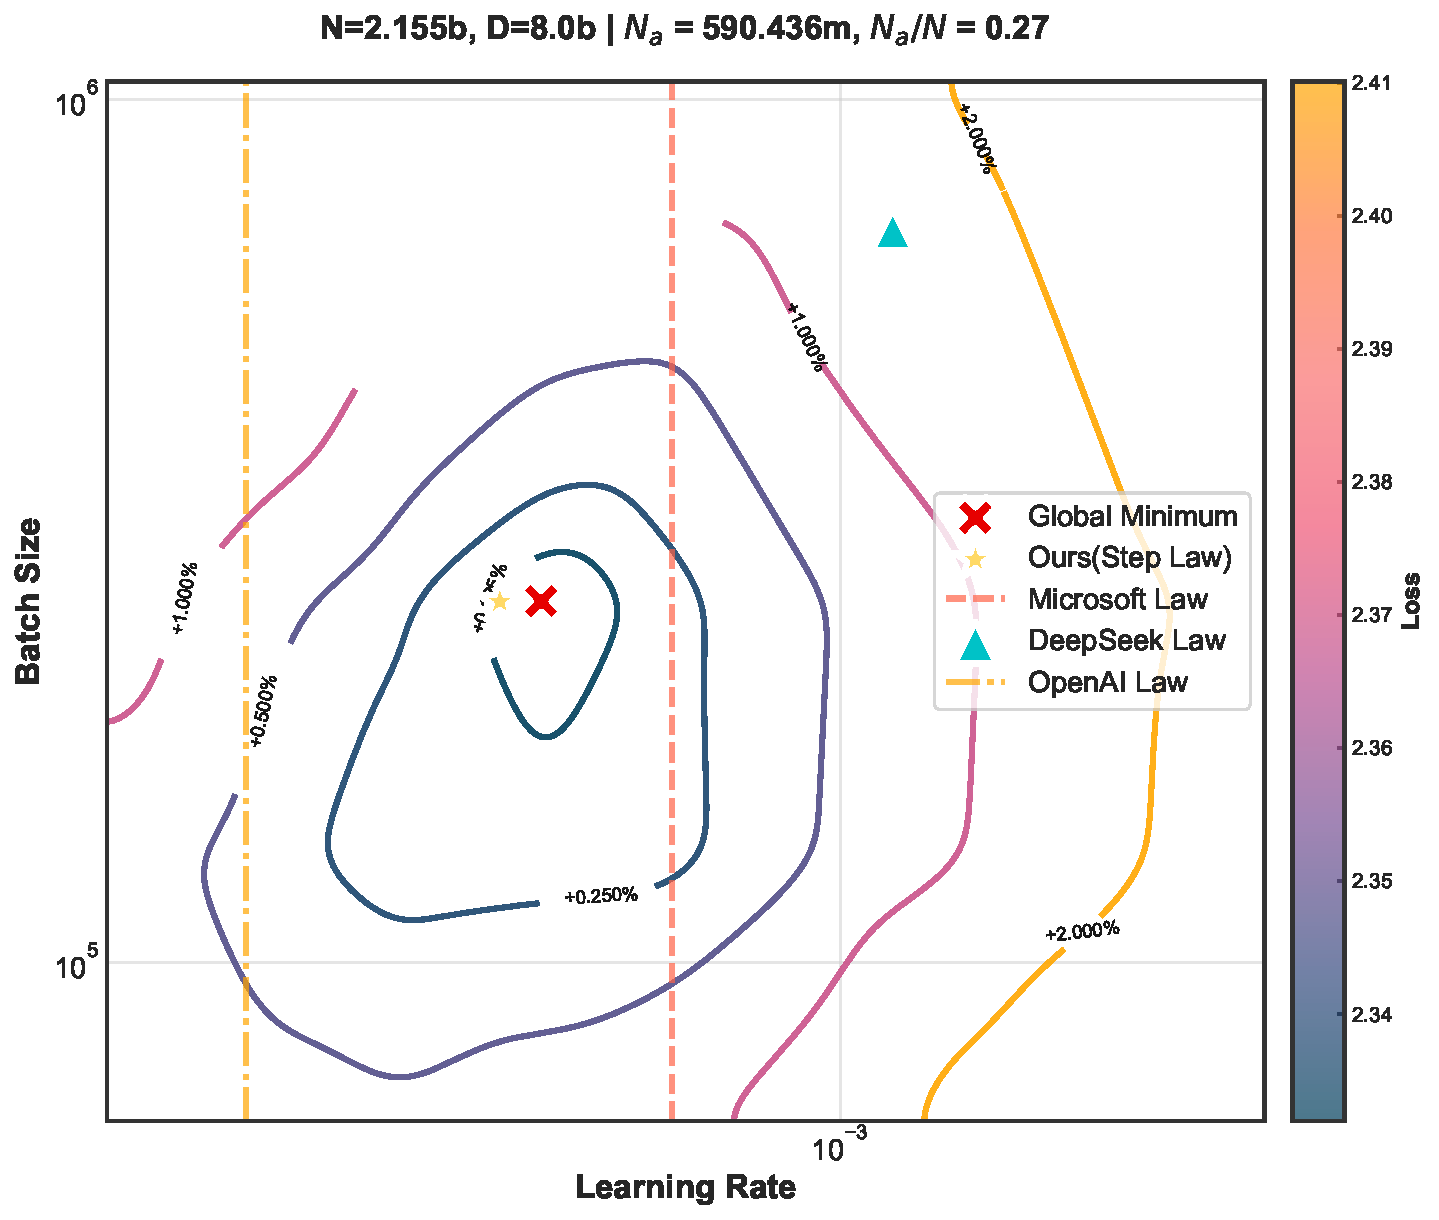
\includegraphics[width=\textwidth]{moe_pics/moe_10.pdf}
        % \caption{1}
        \label{fig:moe_subfig1}
    \end{subfigure}
    \hfill
    \begin{subfigure}[b]{0.3\textwidth}
        \centering
        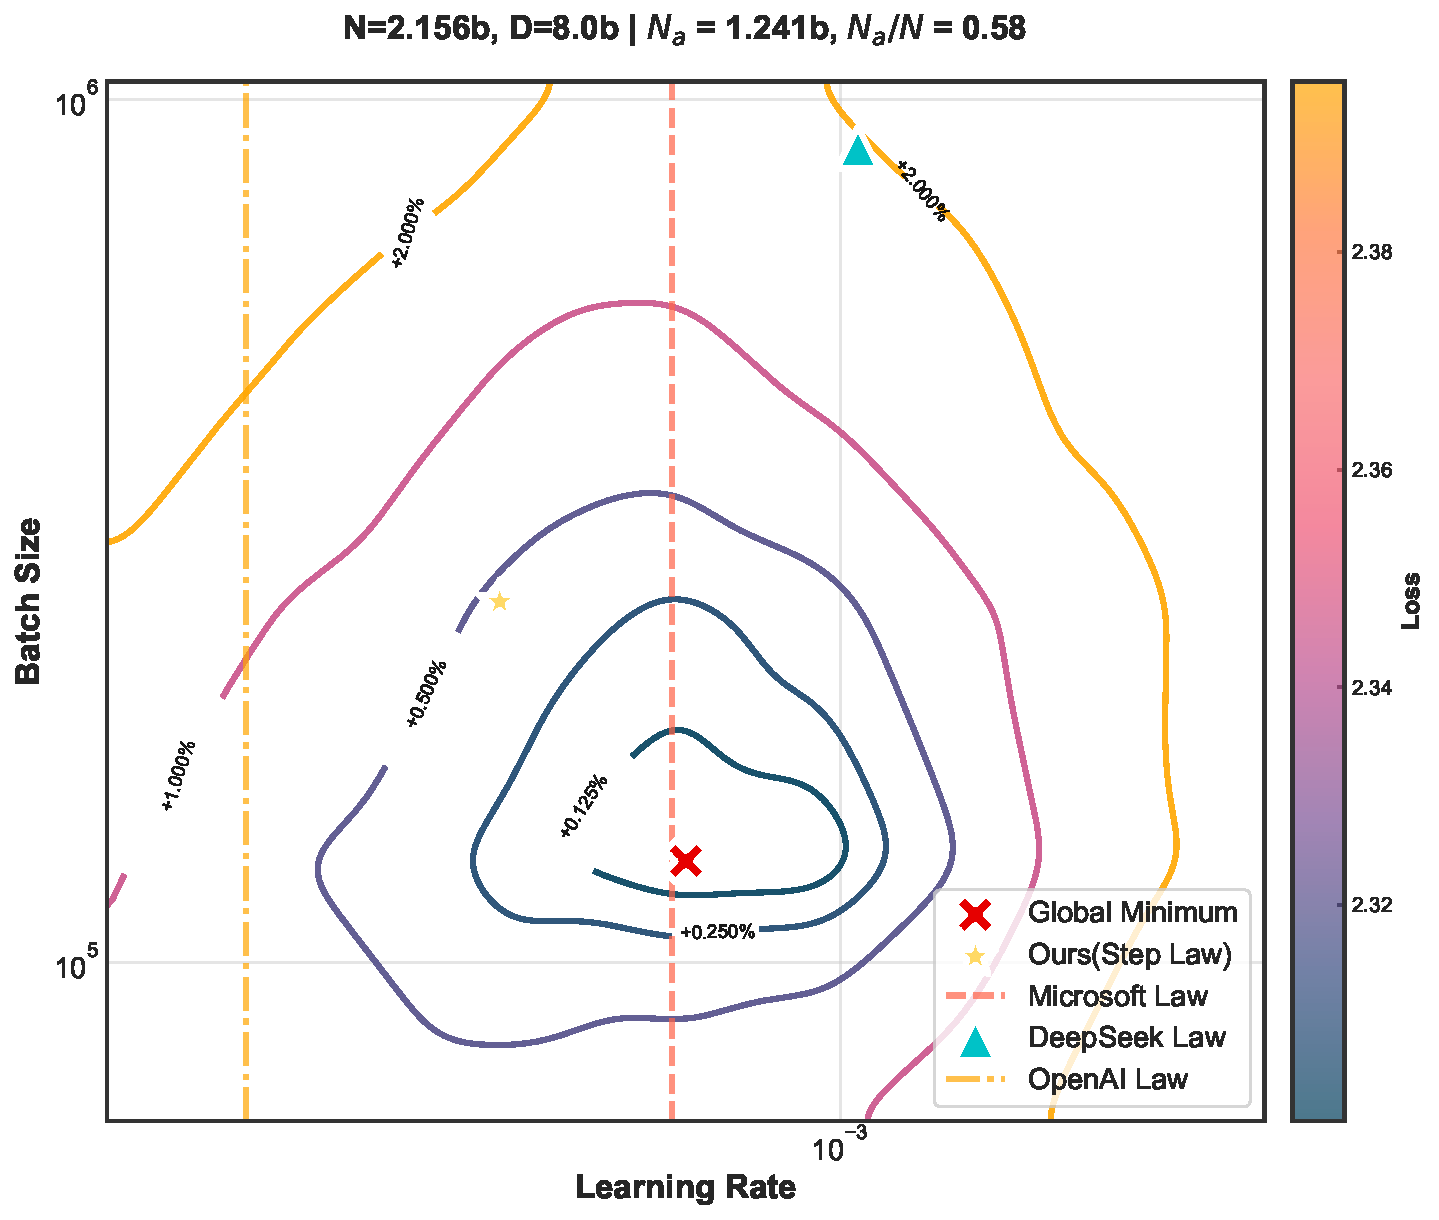
\includegraphics[width=\textwidth]{moe_pics/moe_11.pdf}
        % \caption{2}
        \label{fig:moe_subfig2}
    \end{subfigure}
    \hfill
    \begin{subfigure}[b]{0.3\textwidth}
        \centering
        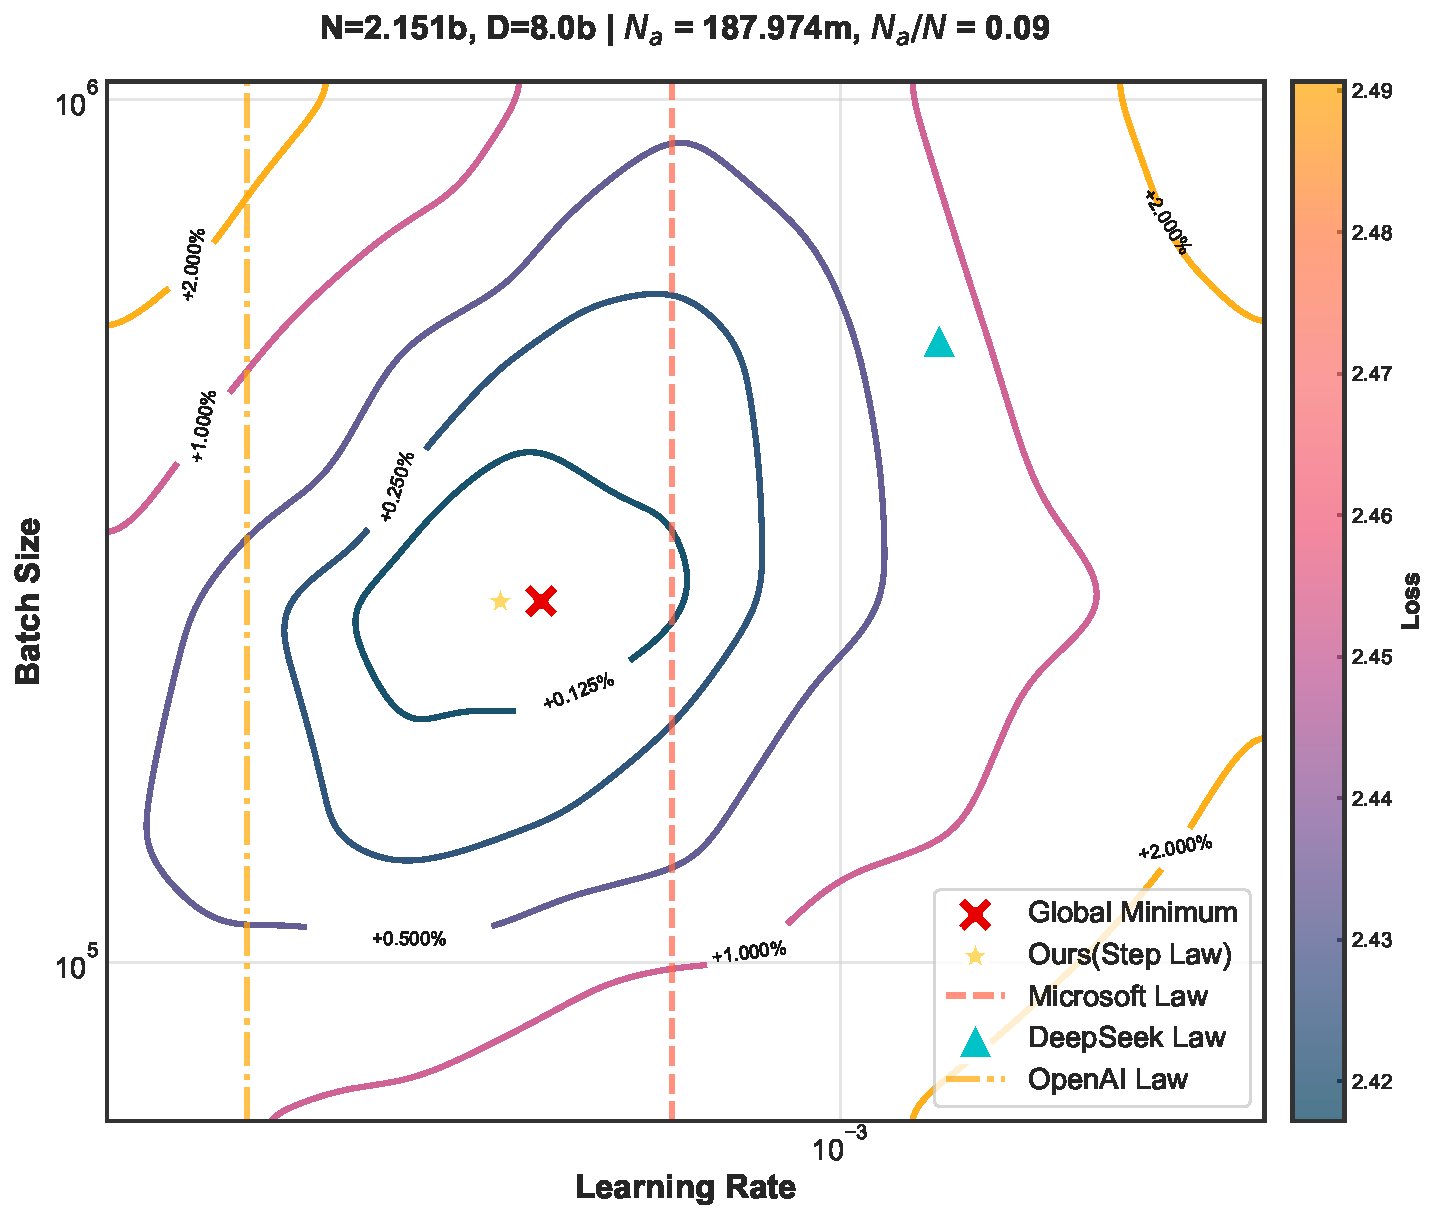
\includegraphics[width=\textwidth]{moe_pics/moe_8.pdf}
        % \caption{3}
        \label{fig:moe_subfig3}
    \end{subfigure}
    \caption{ \textbf{Validation loss landscapes of MoE models under varying sparsity ratios ($ N_a/N $).} Left: Low sparsity ($ N_a/N=0.27 $). Middle: Medium sparsity ($ N_a/N=0.58 $). Right: Medium sparsity at D=8.0B. Our method consistently approximates global minima across sparsity regimes.}
    \label{fig:moe}
\end{figure*}


    \subsection{Data-Distribution Robustness}
    \label{sec:data}

    \begin{figure*}[h!]
    \centering
    \begin{subfigure}[b]{0.3\textwidth}
    \centering
    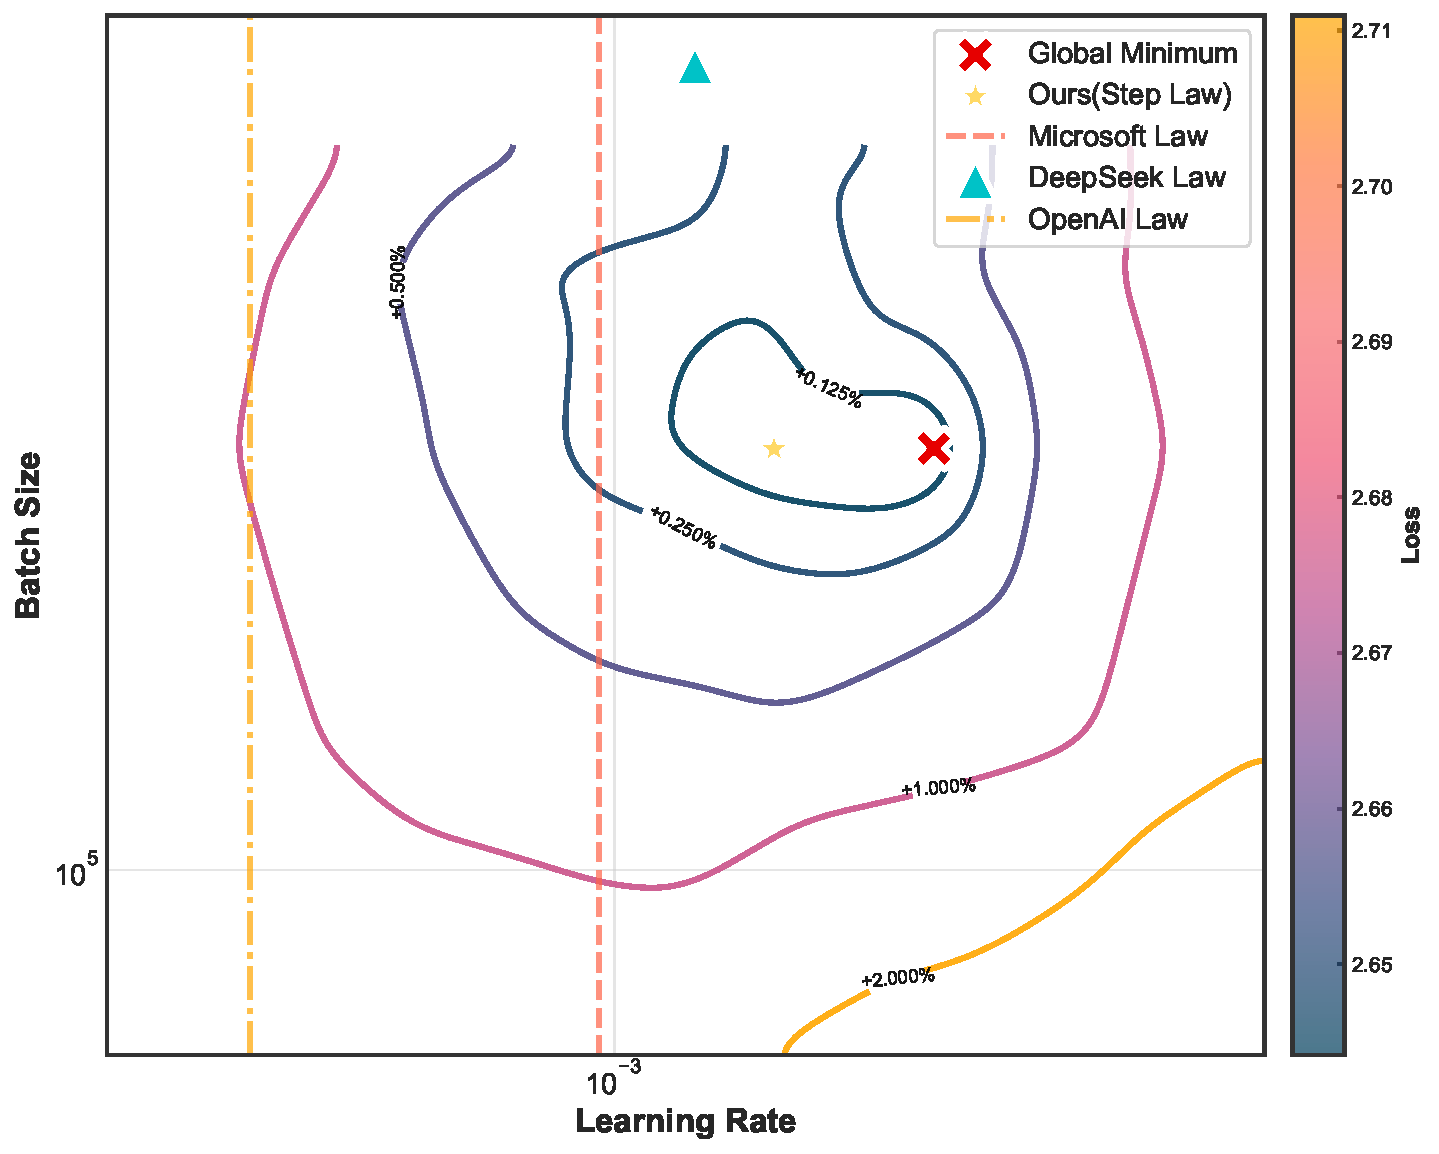
\includegraphics[width=\textwidth]{pics/N429260800_D8000000000_recipebilingual_config_space.pdf}
    \caption{Bilingual Corpus}
    \label{fig:moe_subfig1}
    \end{subfigure}
    \hfill
    \begin{subfigure}[b]{0.3\textwidth}
    \centering
    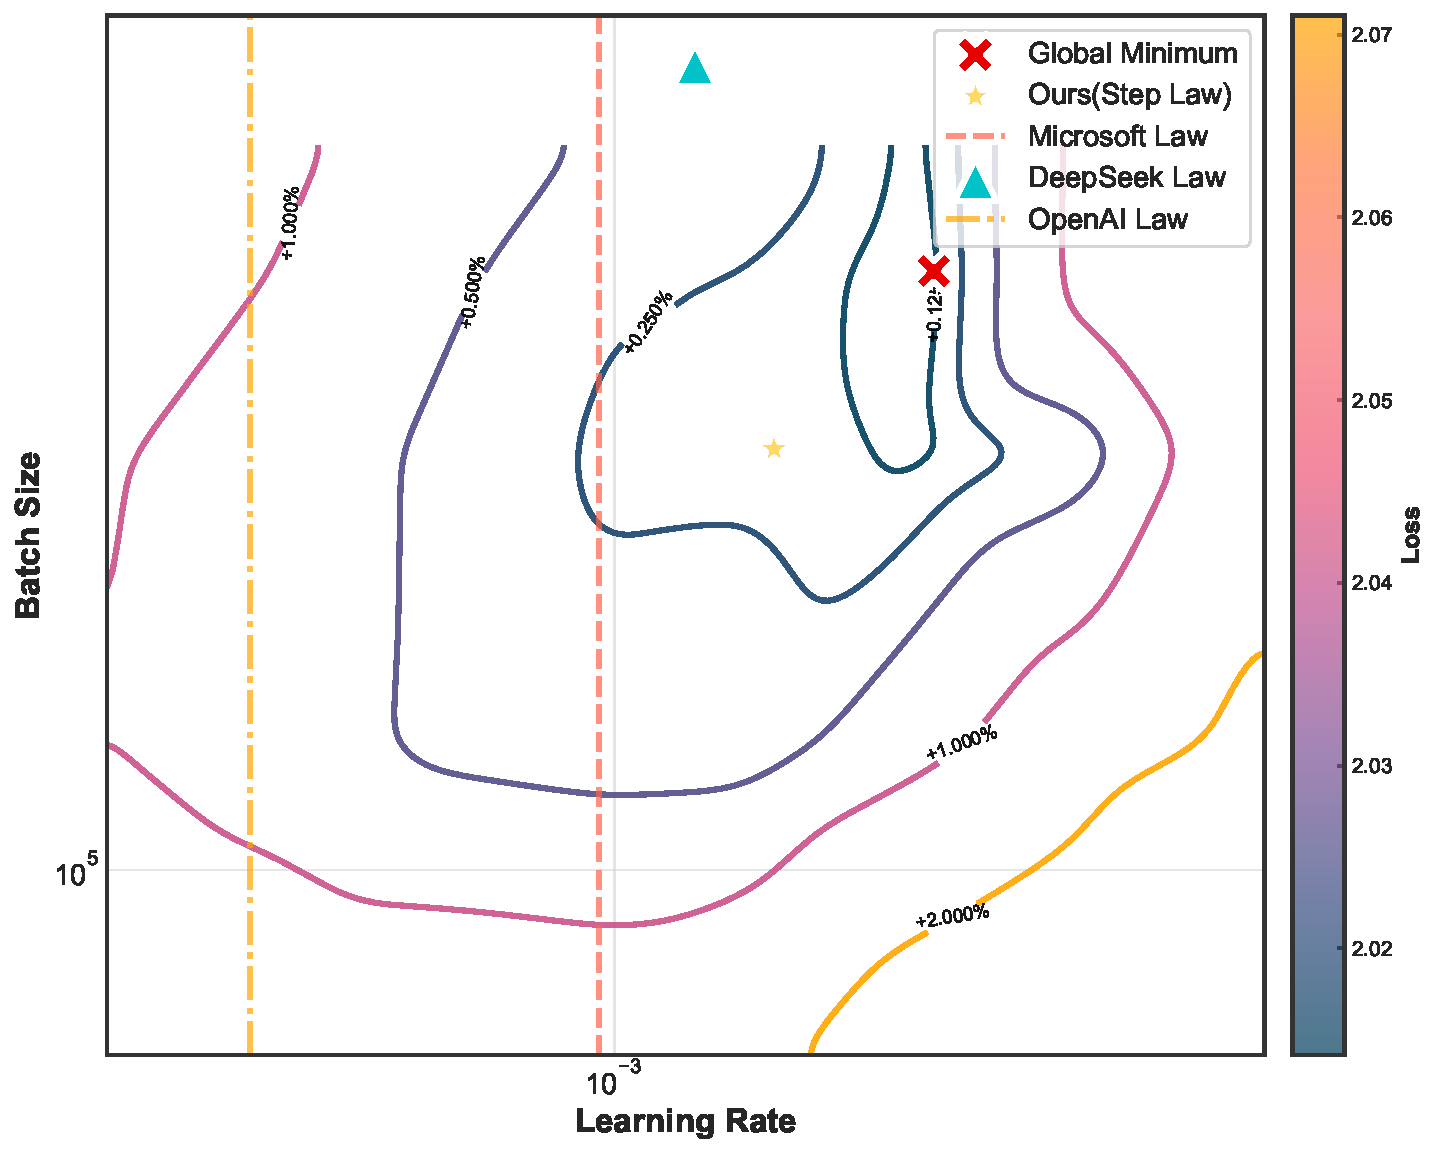
\includegraphics[width=\textwidth]{pics/N429260800_D8000000000_recipecode_config_space.pdf}
    \caption{Code Integration}
    \label{fig:moe_subfig2}
    \end{subfigure}
    \hfill
    \begin{subfigure}[b]{0.3\textwidth}
    \centering
    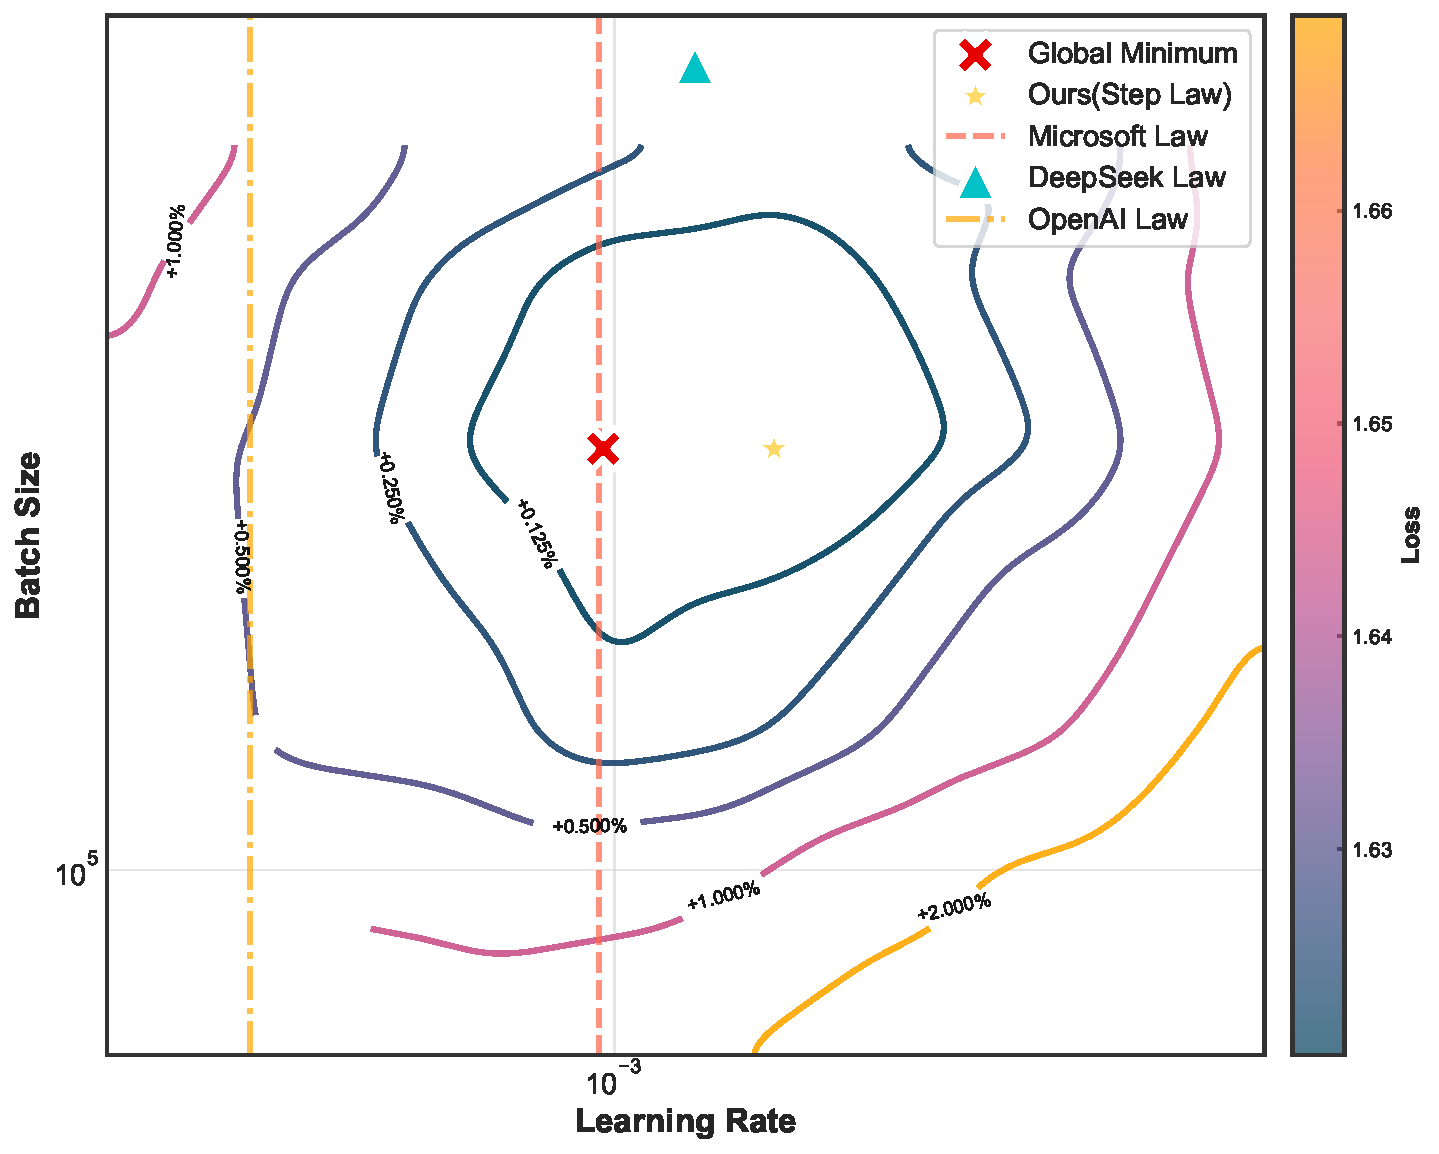
\includegraphics[width=\textwidth]{pics/N429260800_D8000000000_recipemorecode_config_space.pdf}
    \caption{Code-Dominante}
    \label{fig:moe_subfig3}
    \end{subfigure}
    \caption{\textbf{Configuration Space Analysis under Different Data Recipes.} Our method demonstrates stable convergence patterns across varying data compositions.}
    \label{fig:data_distribution}
    \end{figure*}

    To rigorously assess the robustness of our HP scaling law across varied data distributions $\mathbb{D}$, we design three distinct data distributions, progressively diverging from the original composition, as detailed in Appendix Tab.~\ref{tab:data_recipes}:
    \begin{enumerate}
    \item \textbf{Bilingual Corpus:} We augmented the original English-only dataset with Chinese data, creating a bilingual distribution to test the law's validity in multilingual settings.
    \item \textbf{Code Integration:} We reduced English content and incorporated 32.36\% of the code-the-stack dataset, examining the law's adaptability to code-heavy distributions.
    \item \textbf{Code-Dominant:} We further decreased English content and increased code-the-stack to 57.05\%, representing an extreme shift towards code-based data.
    \end{enumerate}
    
    As shown in Fig.~\ref{fig:data_distribution}, our formula maintains remarkable predictive accuracy across all three distributions, with relative prediction errors within 0.25\% of the global minimum. This performance consistently surpasses alternative approaches, which exhibit larger deviations. These results highlight two crucial insights:

    \begin{itemize}
    \item The HP scaling law demonstrates statistical invariance across linguistic and structural changes in the dataset, supporting its generalizability beyond standard natural language distributions.
    
    \item The predicted optimal hyperparameters remain stable even with highly heterogeneous training data, reinforcing our approach's robustness.
    \end{itemize}

    These findings are particularly significant for designing scalable and adaptable training paradigms applicable across diverse deployment scenarios with varying dataset characteristics.


    % TODO 这边改下
    \begin{tcolorbox}
        [callout={Key Takeaways}]
        \begin{enumerate}[\textbullet]
            \item \textbf{Topological Invariance:} Our HP scaling laws exhibit
                statistical invariance in the scaling constants for LR and BS
                with respect to model scale $N$ and data size $D$, even when varying
                topological features of model architectures.

            \item \textbf{Sparsity Independence:} The HP scaling law extends beyond dense Transformers and remains effective for sparse MoE models, with our approach achieving superior prediction accuracy across different sparsity levels, reinforcing the broader applicability of scaling laws in diverse neural architectures $\mathbb{A}$.

            \item \textbf{Data-Distribution Robustness:} The HP scaling law
                shows robustness across diverse data distributions $\mathbb{D}$.
        \end{enumerate}
    \end{tcolorbox}

    \section{Conclusions}
    In this paper, we provide a crucial advancement in efficient hyperparameter
    optimization for LLMs. By empirically unveiling and rigorously validating universal
    scaling laws for learning rate and batch size—underpinned by the discovery of
    loss landscape convexity—we move beyond computationally expensive grid searches
    and limited transfer methods. Our robust HP scaling laws, supported by an unprecedentedly
    large empirical study and open-sourced resources, empower the community with
    a practical and generalizable approach for navigating the hyperparameter
    configuration space in LLM pretraining, thereby facilitating more efficient and
    scalable LLM development.
    
    \section*{Limitations}
    \label{sec:limitation} While our empirical study provides valuable universal
    HP scaling laws and demonstrates their practical efficacy, it is essential
    to acknowledge the limitations inherent in an empirical approach. Our findings
    are primarily data-driven. Future work should focus on developing a more
    theoretical understanding of the observed power-law relationships, potentially
    deriving them from first principles to enhance their predictive power and generalizability
    beyond the empirically validated domain.
    
\section*{Acknowledgments}
The work was supported by National Science and Technology Major Project of China (2023ZD0121300).

    \bibliography{ref_scaling_law}
    \bibliographystyle{acl_natbib}
    
    \appendix
    \section{Appendix}
    \label{sec:appendix}

    \subsection{Model Scale Dominates Optimal Hyperparameter Selection Over
    Computational Complexity}

    \begin{table*}
        [t]
        \centering
        \begin{tabular}{ccccccccc}
            \hline
            $d_{{model}}$ & $d_{{ff}}$  & $N_{{head}}$ & $N_{{layer}}$ & $lr$       & $bs$  & $D$        & $N$        & $M$        \\
            \hline
            \multicolumn{9}{c}{Constant $N$ Experiments} \\
            \hline
            1280                                       & 12264 & 10   & 8    & 1.95E-03 & 262,144 & 8.00E+09 & 4.29E+08 & 2.83E+09 \\
            1280                                       & 6280  & 10   & 14   & 1.38E-03 & 262,144 & 8.00E+09 & 4.29E+08 & 3.02E+09 \\
            1536                                       & 9600  & 12   & 8    & 9.77E-04 & 131,072  & 8.00E+09 & 4.29E+08 & 2.88E+09 \\
            1536                                       & 7264  & 12   & 10   & 1.38E-03 & 262,144 & 8.00E+09 & 4.29E+08 & 2.95E+09 \\
            1536                                       & 4608  & 12   & 14   & 9.77E-04 & 131,072  & 8.00E+09 & 4.29E+08 & 3.10E+09 \\
            2048                                       & 6000  & 16   & 8    & 9.77E-04 & 262,144 & 8.00E+09 & 4.29E+08 & 2.98E+09 \\
            2048                                       & 4256  & 16   & 10   & 9.77E-04 & 262,144 & 8.00E+09 & 4.29E+08 & 3.08E+09 \\
            2048                                       & 2256  & 16   & 14   & 9.77E-04 & 262,144 & 8.00E+09 & 4.29E+08 & 3.28E+09 \\
            \hline
            \multicolumn{9}{c}{Constant $M$ Experiments} \\
            \hline
            1280                                       & 12608 & 10   & 8    & 1.38E-03 & 262,144 & 8.00E+09 & 4.40E+08 & 2.89E+09 \\
            1280                                       & 5888  & 10   & 14   & 1.38E-03 & 262,144 & 8.00E+09 & 4.08E+08 & 2.89E+09 \\
            1536                                       & 9656  & 12   & 8    & 1.38E-03 & 262,144 & 8.00E+09 & 4.31E+08 & 2.89E+09 \\
            1536                                       & 7040  & 12   & 10   & 1.38E-03 & 262,144 & 8.00E+09 & 4.19E+08 & 2.89E+09 \\
            1536                                       & 4056  & 12   & 14   & 9.77E-04 & 262,144 & 8.00E+09 & 3.94E+08 & 2.89E+09 \\
            2048                                       & 5704  & 16   & 8    & 9.77E-04 & 262,144 & 8.00E+09 & 4.15E+08 & 2.89E+09 \\
            2048                                       & 3744  & 16   & 10   & 6.91E-04 & 131,072  & 8.00E+09 & 3.98E+08 & 2.89E+09 \\
            2048                                       & 1504  & 16   & 14   & 6.91E-04 & 131,072  & 8.00E+09 & 3.64E+08 & 2.89E+09 \\
            \hline
        \end{tabular}
        \caption{\textbf{Model configurations for constant $N$ and constant $M$ experiments.}
        The first group (top) maintains constant parameter count $N$ $\approx$ 4.29E+08,
        while the second group (bottom) maintains constant computational complexity
        $M$ $\approx$ 2.89E+09. $M$:  non-embedding FLOPs/token.}
        \label{tab:model_configs}
    \end{table*}

    To investigate how model architecture variations affect optimal hyperparameter
    settings, we conducted two sets of control experiments. In the first set, we
    maintained a constant parameter count ($N$), while in the second set, we kept
    the computational complexity ($M$) constant. Both sets used identical training
    configurations with 8B training tokens, varying only in their architectural
    proportions.

    % TODO 文章里面直接就说我们各采用了8组设定，下面这一段直接注释掉。
    Tab.~\ref{tab:model_configs} presents the detailed configurations and
    results for both experimental groups. For each model, we systematically
    varied the hidden dimension ($d_{{model}}$), feed-forward dimension ($d_{{ff}}$), number of
    attention heads ($N_{{head}}$), and number of layers ($N_{{layer}}$) while maintaining either
    constant $N$ or $M$. The embedding dimension ($D$) was fixed at 8.00E+09 across all
    experiments.

    To visualize the impact of hyperparameters across different architectural configurations,
    we generated heatmaps of the loss landscape with respect to LR and BS in Fig. \ref{fig:Topological_Invariance} and
    \ref{fig:M_shape}. The heatmaps reveal consistent patterns in the optimal
    hyperparameter regions across different architectural configurations within
    each experimental group.


    \begin{figure*}[!t]
        \setlength{\abovecaptionskip}{0pt}
        \setlength{\belowcaptionskip}{10pt}
        %\vskip -0.2in
        \begin{center}
            \centerline{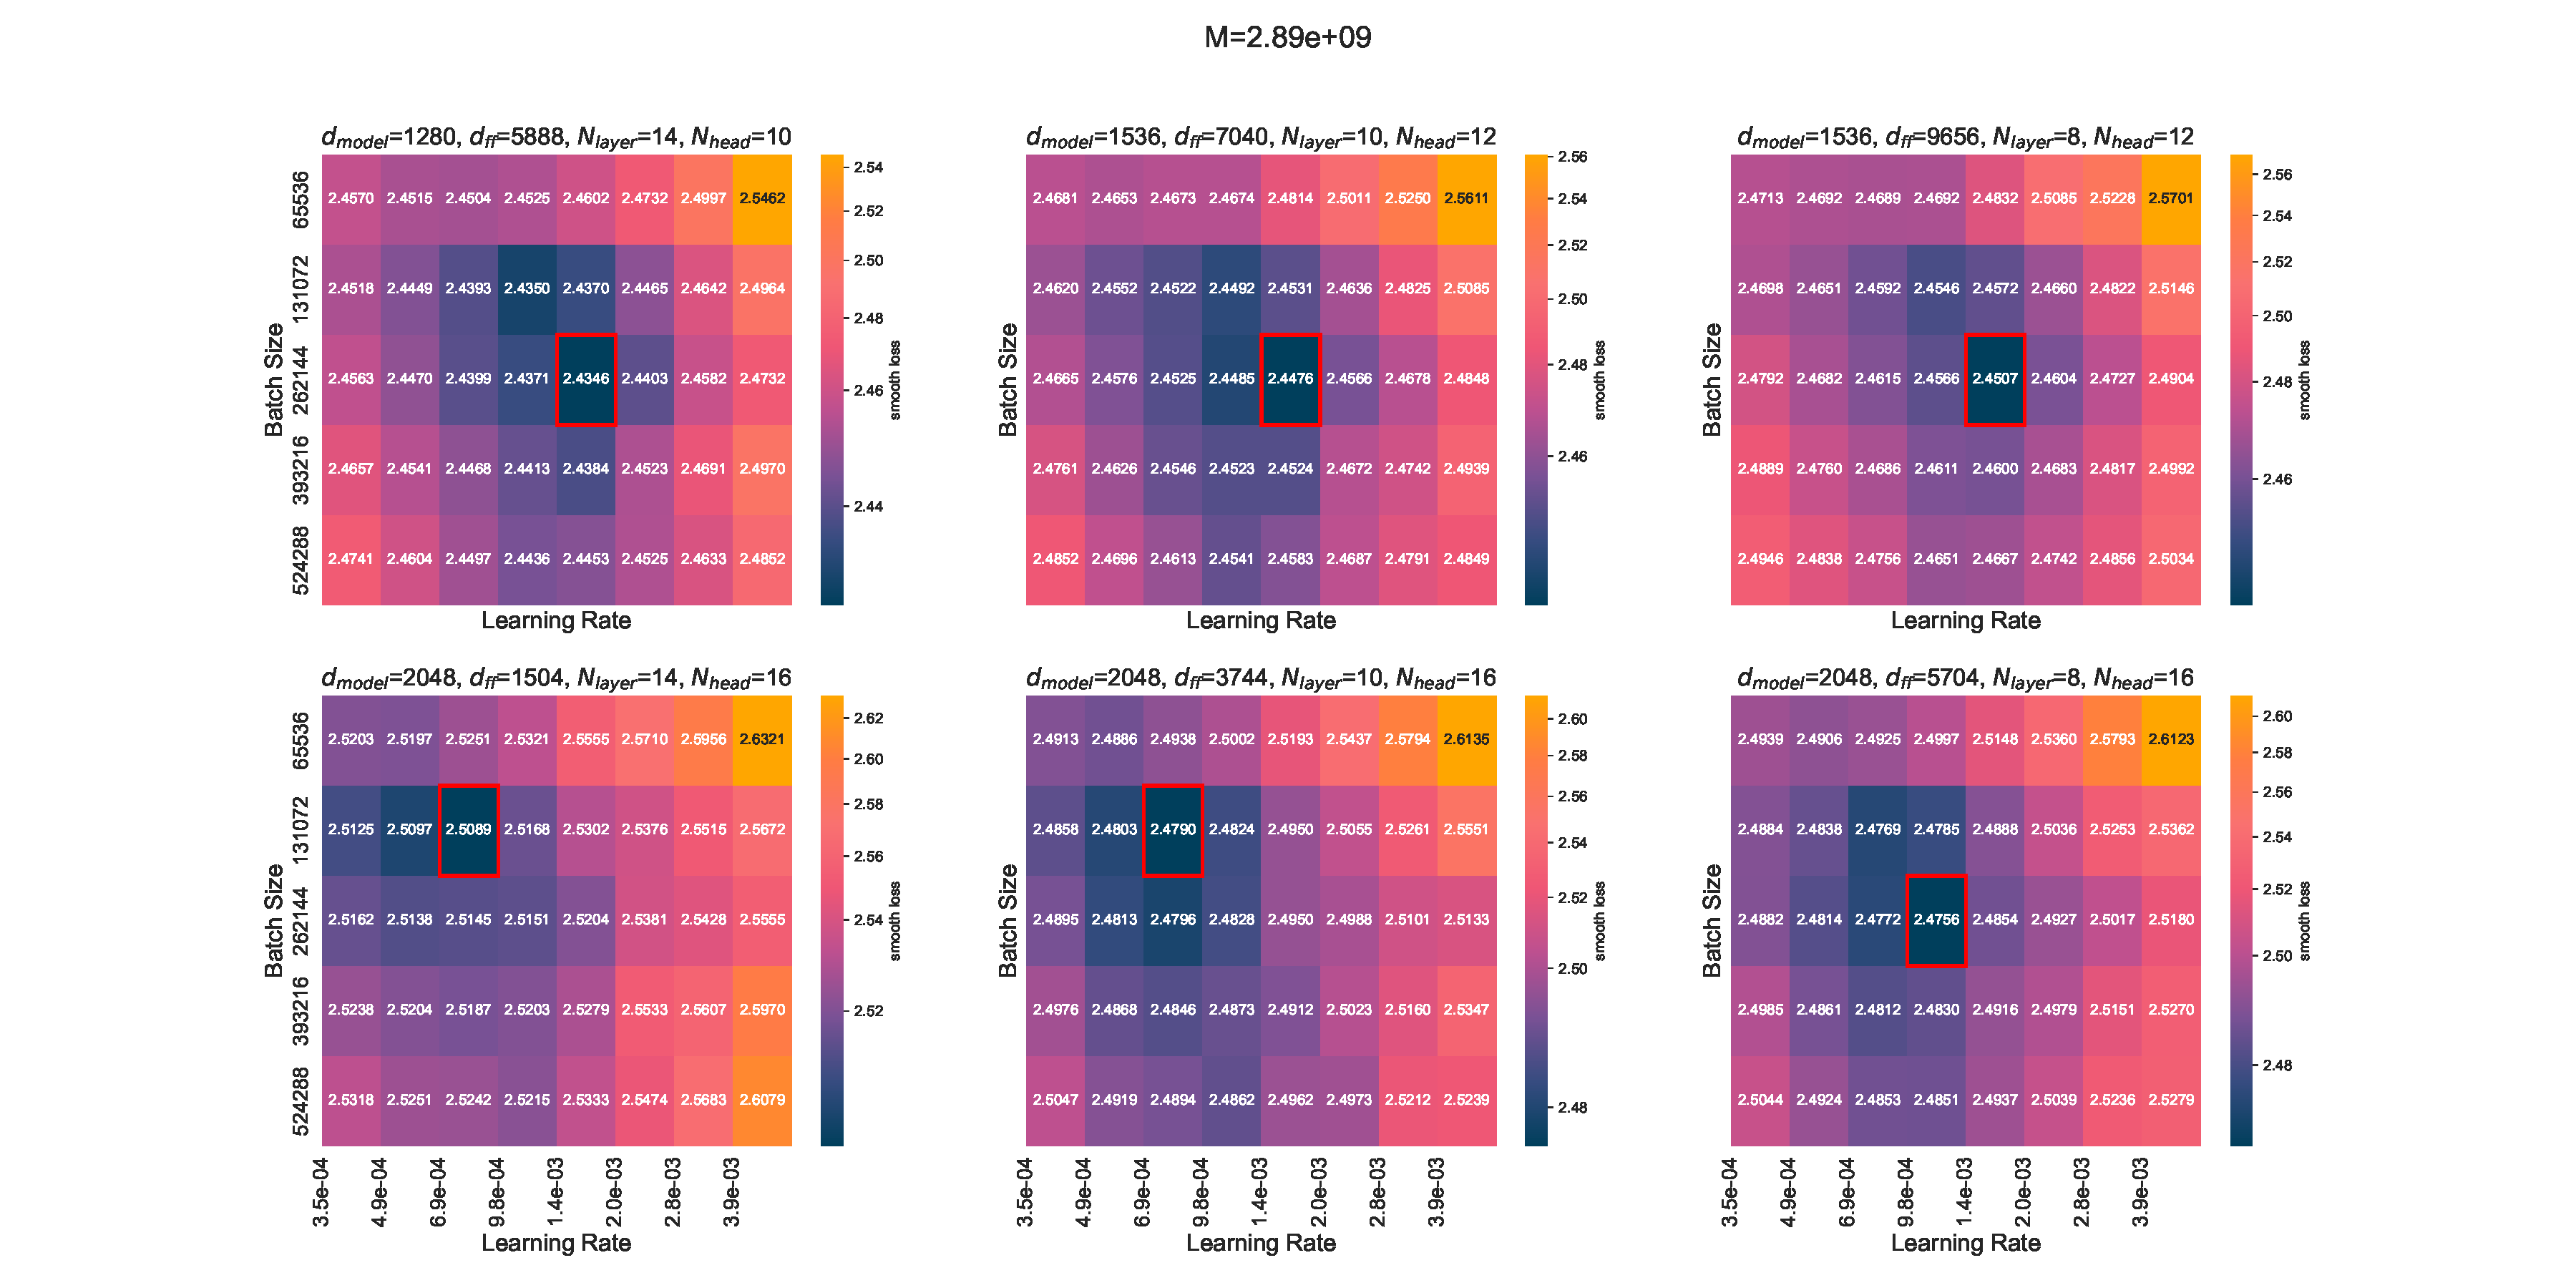
\includegraphics[width=1.0\textwidth,trim=1 10 1 1,clip]{pics/M_shape.pdf}}
            % \vskip -10pt
            \caption{ Loss landscapes visualized as heatmaps across learning rate (x-axis)
        and batch size (y-axis) configurations. Darker colors indicate lower loss
        values. Shows results for models with constant
        computational complexity $M$, exhibiting slightly more variance in optimal
        hyperparameter regions.}
            \label{fig:M_shape}
            % \vskip -30pt
        \end{center}
    \end{figure*}

    The experimental results reveal several key findings: (\rmnum{1}) Models with
    constant $N$ demonstrate remarkably consistent optimal hyperparameter regions,
    with minimal variation in minimum loss values (ranging from 2.4294 to 2.4776)
    despite significant architectural differences. (\rmnum{2}) The constant M
    experiments show slightly more variation in optimal hyperparameter regions
    and minimum loss values (ranging from 2.4346 to 2.5089), suggesting that parameter
    count $N$ may be a more robust indicator for hyperparameter selection than computational
    complexity $M$. (\rmnum{3}) Across both experimental groups, the optimal
    learning rates typically fall within a narrow range (6.91E-04 to 1.95E-03), and
    batch sizes cluster around either 131,072 or 262,144, regardless of the specific
    architectural configuration.


    These findings strongly suggest that the fundamental scale metrics,
    particularly the parameter count $N$, are more influential in determining optimal
    hyperparameter settings than specific architectural choices. This
    observation motivates our discussion of hyperparameter scaling laws in
    relation to $N$ in Section~\ref{fitting_hp_scaling_law}.

    \subsection{Model Structural Parameters And Results}

    \label{app:struct}

\begin{table*}[h!]
    \centering
    \begin{tabular}{ccccccc}
        \toprule Model & {$N$} & {$D$} & $d_{{model}}$ & $d_{{ff}}$ & $N_{{head}}$ & $N_{{layer}}$ \\
        \midrule 
        0 & 2.15E+08 & 1.14E+10 & 960 & 9368 & 15 & 7 \\
        1 & 4.29E+08 & 5.00E+10 & 1280 & 9472 & 10 & 10 \\
        2 & 2.68E+08 & 8.00E+10 & 1024 & 9552 & 16 & 8 \\
        3 & 4.29E+08 & 8.00E+09 & 1280 & 9472 & 10 & 10 \\
        4 & 1.07E+09 & 2.00E+10 & 2048 & 8192 & 16 & 16 \\
        5 & 5.37E+08 & 1.00E+10 & 1280 & 9048 & 10 & 13 \\
        6 & 2.15E+08 & 4.00E+09 & 960 & 9368 & 15 & 7 \\
        7 & 2.68E+08 & 5.00E+09 & 1024 & 9552 & 16 & 8 \\
        8 & 2.68E+08 & 1.42E+10 & 1024 & 9552 & 16 & 8 \\
        9 & 1.07E+09 & 5.69E+10 & 2048 & 8192 & 16 & 16 \\
        10 & 2.15E+08 & 1.00E+11 & 960 & 9368 & 15 & 7 \\
        11 & 4.29E+08 & 2.27E+10 & 1280 & 9472 & 10 & 10 \\
        12 & 5.37E+08 & 2.84E+10 & 1280 & 9048 & 10 & 13 \\
        13 & 2.15E+08 & 2.00E+10 & 960 & 9368 & 15 & 7 \\
        14 & 4.29E+08 & 4.00E+10 & 1280 & 9472 & 10 & 10 \\
        15 & 2.68E+08 & 2.50E+10 & 1024 & 9552 & 16 & 8 \\
        16 & 5.37E+08 & 5.00E+10 & 1280 & 9048 & 10 & 13 \\
        17 & 1.07E+09 & 1.00E+11 & 2048 & 8192 & 16 & 16 \\
        \bottomrule
    \end{tabular}
    \caption{\textbf{Dense Model Configuration.}} % 表格标题
    \label{tab:struct}
\end{table*}


        \begin{table*}
        [h!]
        \centering

\begin{tabular}{cccccccccc}
\toprule
Model & {$N$} & {$D$} & {$d_{{model}}$} & {$N_{{head}}$} & {$N_{{layer}}$} & {$N_{{expert}}$} & {$d_{{moe}}$} & {Top-$k$} & {$N_a$} \\
\midrule
0 & 2150612992 & 2000000000 & 1408 & 11 & 16 & 89 & 352 & 1 & 187973632 \\
1 & 2150612992 & 2000000000 & 1408 & 11 & 16 & 88 & 352 & 2 & 232579072 \\
2 & 2155174912 & 2000000000 & 1408 & 11 & 16 & 8 & 3528 & 1 & 590436352 \\
3 & 2156188672 & 2000000000 & 1408 & 11 & 16 & 8 & 2888 & 3 & 1241270272 \\
4 & 2150612992 & 4000000000 & 1408 & 11 & 16 & 89 & 352 & 1 & 187973632 \\
5 & 2150612992 & 4000000000 & 1408 & 11 & 16 & 88 & 352 & 2 & 232579072 \\
6 & 2155174912 & 4000000000 & 1408 & 11 & 16 & 8 & 3528 & 1 & 590436352 \\
7 & 2156188672 & 4000000000 & 1408 & 11 & 16 & 8 & 2888 & 3 & 1241270272 \\
8 & 2150612992 & 8000000000 & 1408 & 11 & 16 & 89 & 352 & 1 & 187973632 \\
9 & 2150612992 & 8000000000 & 1408 & 11 & 16 & 88 & 352 & 2 & 232579072 \\
10 & 2155174912 & 8000000000 & 1408 & 11 & 16 & 8 & 3528 & 1 & 590436352 \\
11 & 2156188672 & 8000000000 & 1408 & 11 & 16 & 8 & 2888 & 3 & 1241270272 \\
12 & 2150612992 & 20000000000 & 1408 & 11 & 16 & 89 & 352 & 1 & 187973632 \\
13 & 2150612992 & 20000000000 & 1408 & 11 & 16 & 88 & 352 & 2 & 232579072 \\
14 & 2155174912 & 20000000000 & 1408 & 11 & 16 & 8 & 3528 & 1 & 590436352 \\
15 & 2156188672 & 20000000000 & 1408 & 11 & 16 & 8 & 2888 & 3 & 1241270272 \\
\bottomrule
\end{tabular}
        \caption{\textbf{MoE Model Configuration.} {$N_{{expert}}$} denotes the number of experts. {$d_{{moe}}$} denotes the hidden size of experts. 
 {Top-$k$} denotes the number in the routing algorithm. {$N_a$} denotes the activate parameters.} % 表格标题
        \label{tab:moe_struct}
        \end{table*}

    \begin{table*}[h!]
 
    \small
    \centering
    \begin{tabular}{lccccc}
    \toprule
    \textbf{Dataset} & \textbf{Baseline} & \textbf{Code+Math} & \textbf{More Code+Math} & \textbf{En-CN} \\
    \midrule
    web-data-en & \centering 79.53 & 44.75 & 20.00 & 44.99 \\
    web-data-cn & -- & -- & -- & 34.52 \\
    code-the-stack & 4.62 & 32.36 & 57.05 & 4.63 \\
    web-data-math & -- & 7.07 & 7.07 & -- \\
    book-non-novel-en & 4.35 & 4.34 & 4.34 & 4.35 \\
    paper & 3.38 & 3.37 & 3.37 & 3.38 \\
    wikipedia-mtlg & 3.24 & 3.24 & 3.24 & 3.25 \\
    stackexchange & 2.21 & 2.21 & 2.21 & 2.22 \\
    wikipedia-en & 1.69 & 1.69 & 1.69 & 1.69 \\
    book-novel-en & 0.83 & 0.83 & 0.83 & 0.83 \\
    wikipedia-cn & 0.13 & 0.13 & 0.13 & 0.13 \\
    \bottomrule
    \end{tabular}
    \caption{\textbf{Comparison of dataset weights (\%) across different training recipes.} Each recipe represents a different focus: baseline, enhanced code and mathematics capability, and English-Chinese bilingual ability. }
    \label{tab:data_recipes}
    \end{table*}
    
    \foreach \i in {0,...,17} {
      \begin{figure}[h!]
        \centering
        \includegraphics[width=0.5\textwidth]{compare_pics/\i.pdf}
        \caption{Illustration of Hyperparameter Configuration Space for  Model \i.}
        \label{fig:compare_\i}
      \end{figure}
    }

    % 插入 moe_pics 下的图片（moe_0 到 moe_11）
    \foreach \i in {0,...,15} {
      \begin{figure}[h!]
        \centering
        \includegraphics[width=0.5\textwidth]{moe_pics/moe_\i.pdf}
        \caption{Illustration of Hyperparameter Configuration Space for MoE Model \i.}
        \label{fig:moe_\i}
      \end{figure}
    }
\end{document}